% % % % % % % % % % % % % % % % % % % % % % % % % % % % % % % % % % % % % % % % %
% INTRO
% % % % % % % % % % % % % % % % % % % % % % % % % % % % % % % % % % % % % % % % %
\section{Time box 7}

\subsection{Time box planning}

\begin{figure}[H]
	\begin{centering}
		%\missingfigure{Updated timebox figure}
		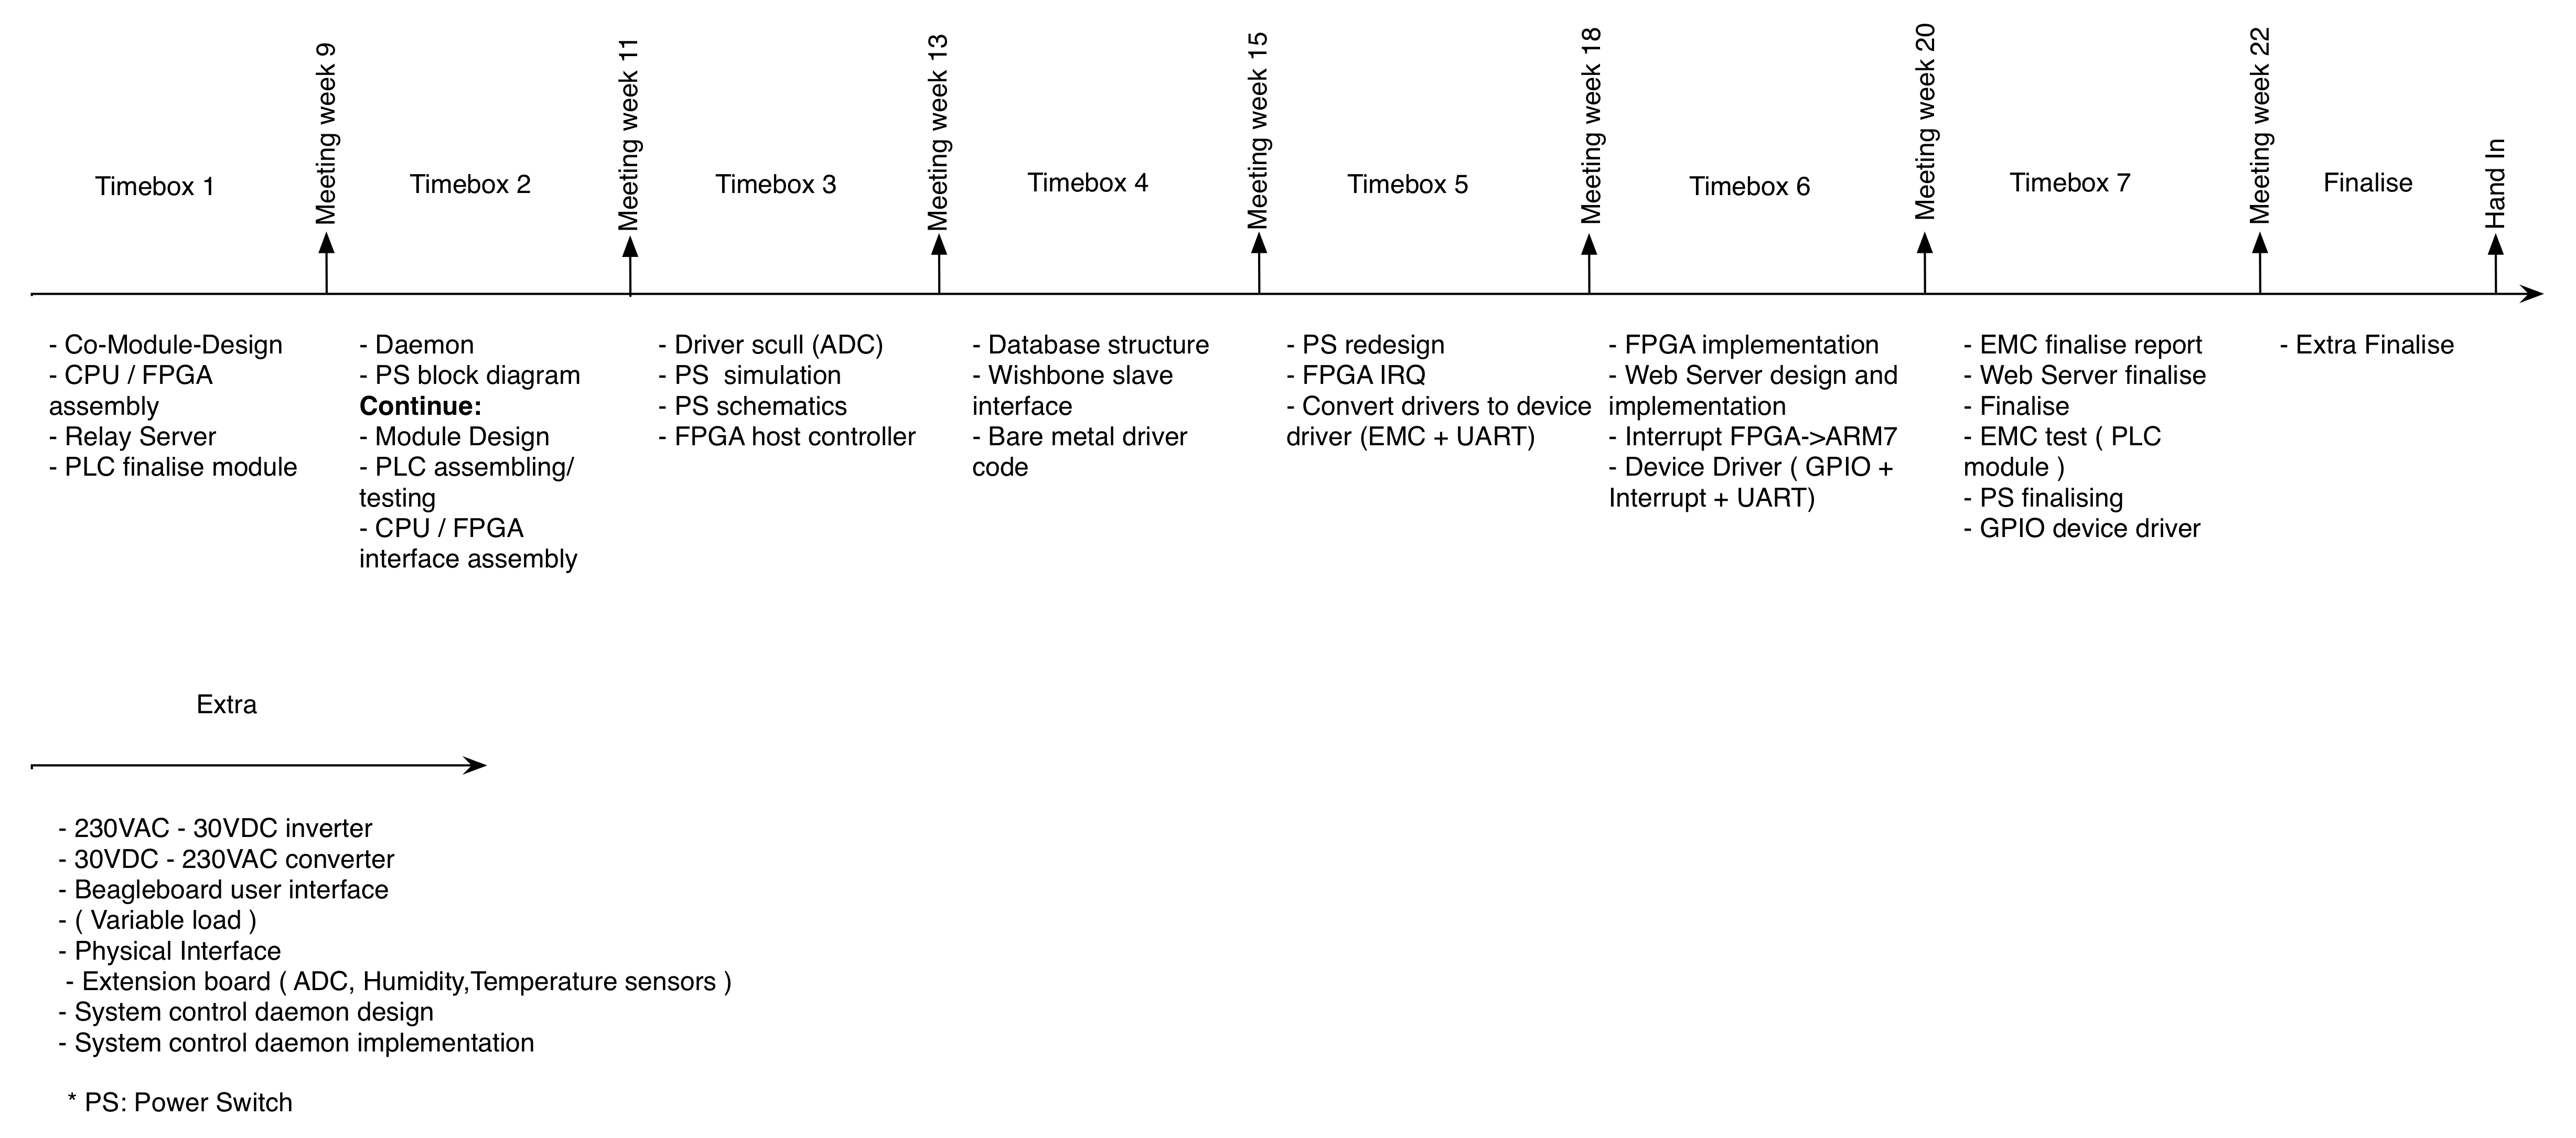
\includegraphics[width=1.0\textwidth]{images/tb_r7.png}
		\caption{Updated time-box}
	\end{centering}
\end{figure}

\subsubsection{Work to be done in this time box}

\begin{itemize}
	\item Requirements for debouncing
	\begin{itemize}
		\item Stability of switches
		\item Time limits
	\end{itemize}
	\item Verification
	\begin{itemize}
		\item External memory controller
		\item Verification of the Spartan 6
	\end{itemize}
	\item Power Switch system
		\begin{itemize}
			\item Testing
		\end{itemize}
	\item Web Interface
		\begin{itemize}
			\item Database Corrections
			\item Error Handling
			\item User experience
		\end{itemize}
	\item GPIO Device driver
	\begin{itemize}
		\item Setup and control of GPIO pins used in the system
	\end{itemize}
\end{itemize}

\paragraph{Description:}

\begin{description}
	\item[Requirements for debouncing] This is the timing requirements for the switch block to avoid bouncing when switching state
	\item[Verification] This is verification of the VHDL design including the EMC part in the LPC2478
	\item[Power Switch system] Verification on the power switch system
	\item[Web Interface] User web interface development.
	\item[GPIO device driver] Driver to set and read the GPIO pins used in the energy HUB system. 
\end{description}

\subsubsection{Time planning}

\begin{table}[H]
\centering
	\begin{tabular}{|l|c|c|c|c|c|}
		\hline
		~			& Requirements	& Verification	& Web Interface  	& Power Switch 	& GPIO \\
		~			& for denouncing	& ~ 			& ~				& Verification		& device driver \\\hline
		Estimation	& 3				& 7			& 35		     		&	3			& 10			\\
		Actual		& 3 				& 15			& 40		     		&	5			& 14			\\
		Developer	& Theis			& Theis		& Paulo			&	Paulo		& Dennis		\\
		\hline
	\end{tabular}
	\caption{Estimation and actual time used on the project}
\end{table}
% % % % % % % % % % % % % % % % % % % % % % % % % % % % % % % % % % % % % % % % %
% % % % % % % % % % % % % % % % % % % % % % % % % % % % % % % % % % % % % % % % %
% Theis Thing
% % % % % % % % % % % % % % % % % % % % % % % % % % % % % % % % % % % % % % % % %
\subsection{Requirements for debouncing - Theis}
%			Intro
%					verification specification
%					deployment specification
%
This section is requirement update for the Switch block from section \ref{sec:Switch interrupt}.
\subsubsection{Analysis}
%			Analysis
%
%                Refactored block diagram
%                Refactored class diagram
%                Detailed use cases
%                User interface specification
%                System interface specification
%                Dimensioning specification 
%
In order to figure out how long the switches is bouncing, some measurement has been made on the switches, while it is shifted. The result is shown below.
\begin{figure}[H]
	\begin{centering}
		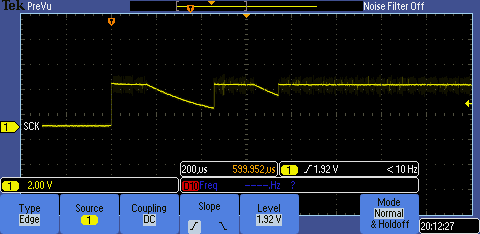
\includegraphics[width=0.7\textwidth]{images/debon_LtoH.png}
		\caption{Signal from switch. Low to high}
	\end{centering}
\end{figure}
From the figure above it is clear that the switch is bouncing, and it is possible to see how long it takes the switch to be stable. From the measurements it takes around $750\mu s$.
\begin{figure}[H]
	\begin{centering}
		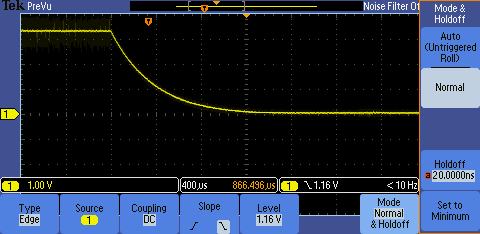
\includegraphics[width=0.7\textwidth]{images/debon_HtoL.png}
		\caption{Signal from switch. High to low}
	\end{centering}
\end{figure}
The figure above shows the switch signal from high to low, this signal is now bouncing, and would not cause any problem because the slope is negative at all time, so when the signal hits the point where the Spartan 6 is switching, the signal would not trigger a switch back. But is takes around $1200\mu s$ for the switch to stabilise.
\subsubsection{Design}
%       	 Design
%
%                UML/SysML deployment view(s)
%                Mechanical specifications and dimensioning
%                HW module specification per block
%                UML SW deployment view
%                Class specification
%                Refactored class diagram
%                Use case scenarios specifications
%                Sequence diagrams
%
In order to remove any debouncing on the switches, a delay is needed. In this system the time has to be the double plus one bit. From the measurements the longest time is $1200\mu s$, the double of that is $2400\mu s$. Calculations for the delay is shown below.
\begin{align}
	t &=	1200\mu s \cdot 2 \\
	f &=	100MHz\\
	t &=	2^{n}\cdot \dfrac{1}{f}\\
	n &=	\dfrac{\ln(f\cdot t)}{\ln(2)}\\
	n &=	\dfrac{\ln(100MHz\cdot 2400\mu s)}{\ln(2)}\\
	n &=	17.87
\end{align}
The bit length for the double delay is 18 and plus 1 bit, a 19 bit vector has to be used in the delay. The delay for 19 bit vector is.
\begin{align}
	t &=	2^{19}\cdot \dfrac{1}{100MHz}\\
	t &=	5.243 ms\\
\end{align}
This is the time delay that is used to debounce the switches.
\subsubsection{Conclusion}
This time delay has been tested in timebox 6 and it is working with the interrupt register in the Spartan 6.
%
%
%
% % % % % % % % % % % % % % % % % % % % % % % % % % % % % % % % % % % % % % % % %
\subsection{Verification - Theis}
%			Intro
%					verification specification
%					deployment specification
%
From the former timeboxes the blocks in the Spartan 6 has been implemented to make a complete system, which is communicating with the external memory controller in the LPC2478.
\subsubsection{External memory controller}
The EMC interface has been analysed with timings and signal assignment in order to make the Spartan 6 read and write data on the right time. On the figure below a block diagram for the EMC in the LPC2478 is shown. The data and pictures is taken from the \textit{LPC24xx user manual}\footnote{\url{http://www.nxp.com/documents/user\_manual/UM10237.pdf}} and the \textit{electrical datasheet}\footnote{\url{http://www.nxp.com/documents/data\_sheet/LPC2478.pdf}} for the LPC2478
\begin{figure}[H]
	\begin{centering}
		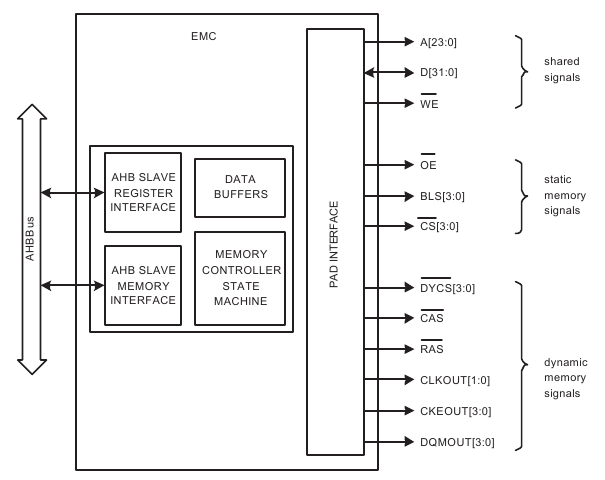
\includegraphics[width=0.8\textwidth]{images/tb7_EMC_block.png}
		\caption{EMC block}
	\end{centering}
\end{figure}
The EMC is used in static mode without the \textit{BLS}\footnote{Byte lane selects} signal, and for memory selection it is only using the \textit{CS2}\footnote{Chip Select 2} for the Spartan 6, this is the interface that has to be implemented in the Spartan 6 to control the wishbone master. The block that takes care of this assignment is the host controller from timebox 3. The timings and signal assignment is shown on the next two figures.
\begin{figure}[H]
	\begin{centering}
		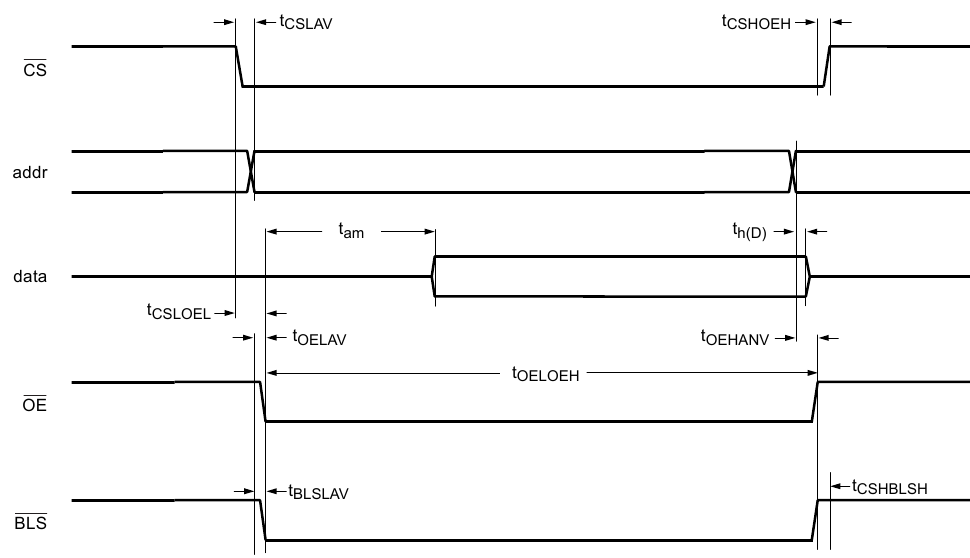
\includegraphics[width=0.8\textwidth]{images/tb7_EMC_read.png}
		\caption{EMC Read timing}
	\end{centering}
\end{figure}
The important thing when the EMC reads data from the Spartan 6, is the $t_{am}$, which is where the EMC reads the data from the Spartan 6, therefore the Spartan 6 has to have valid data ready latest at that time, for the EMC to read correct data. From the electrical datasheet the timing for $t_{am}$ is taken.
\begin{align}
t_{am}min &= (WAITRD - WAITOEN + 1) \cdot T_{cy} - 12.70ns\\
t_{am}typ &= (WAITRD - WAITOEN + 1) \cdot T_{cy} - 9.57ns\\
t_{am}max &= (WAITRD - WAITOEN + 1) \cdot T_{cy} - 8.11ns
\end{align}
The \textit{WAITRD} and \textit{WAITOEN} is integer values that is set in the setup of the EMC in the LPC2478, \textit{WAITRD} has influence on the timing of $t_{am}$ and \textit{OELOEH} increasing this value increase the timing. When \textit{WAITOEN} is increased \textit{CSLOEL} is increased to and $t_{am}$ and \textit{OELOEH} is decreased. The $T_{cy}$ is the time of the clock period.
\begin{align}
CCLK &= 72MHz\\
T_{cy} &= \dfrac{1}{CCLK}\\
T_{cy} &= 13.889ns
\end{align}
The exact timing of $t_{am}$ is calculated late with the Bus functional module used for verification of the Spartan 6 design.
\begin{figure}[H]
	\begin{centering}
		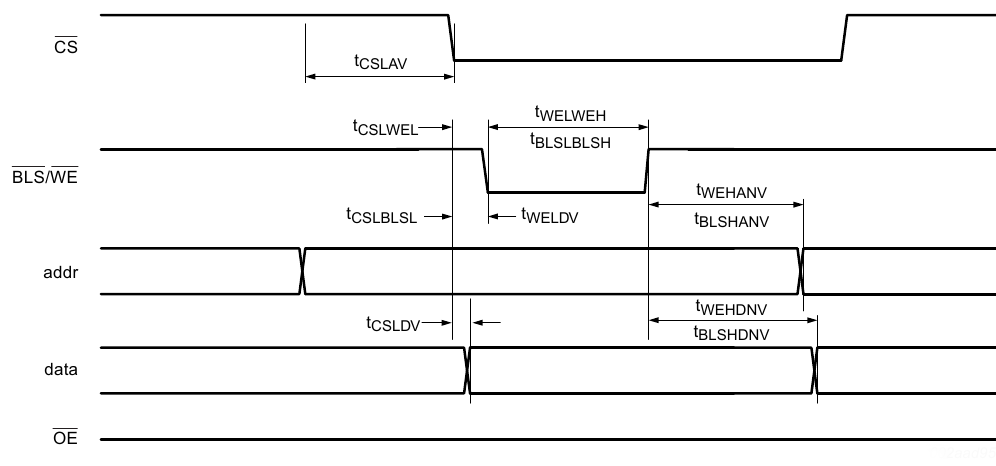
\includegraphics[width=0.8\textwidth]{images/tb7_EMC_write.png}
		\caption{EMC Write timing}
	\end{centering}
\end{figure}
The write diagram shows that the data is valid at the same time as \textit{WE}\footnote{Write Enable} is set low, as long as the Spartan 6 is reacting on \textit{CS2} and the \textit{WE} invalid data is not a problem.
\subsubsection{Bus functional module}
The bus functional module is a module written in VHDL for test purpose. A BFM is able to simulate different interfaces, depending on the code. In this project the BFM is used to test the total design of the Spartan 6 by simulating the EMC interface from the LPC2478. A rough code sketch was handed out from Morten Opprud Jakobsen, timing tweaks needed to be updated in order to make a correct simulation.\\
\dirtree{%
.1 \textcolor{blue}{sim}. 
.2 arm\_emc\_package.vhd. 
.2 \textcolor{blue}{log}. 
.3 arm7\_bfm\_log.txt. 
.2 \textcolor{blue}{stim}. 
.3 arm7\_bfm\_stim.dat. 
.2 tb\_ARM\_BFM.vhd. 
.2 txt\_util.vhd\\. 
}
The file structure of the BFM is shown above, in \textit{arm\_emc\_package.vhd} all the timings and constants is contained. This file also holds the functions for a read and write cycle, with signal assignment in the correct order and time from the timings. \textit{txt\_util.vhd} holds function for converting text strings. The \textit{tb\_ARM\_BFM.vhd} is the test bench file, this file takes a data input from the data file. The data file tells the BFM what to do, if it shall read, write, wait or log something, the logs is written to the log file. The BFM is used on the final Spartan 6 design with the following data file.
\begin{lstlisting}[caption=BFM data file]
#WAIT 10
#LOG Write 0x00 to LEDs
#WR 0000000000010000 0000000000000000
#LOG Change switches
#SW 01000000
#WAIT 30
#LOG Read IRQ reg
#RD 0000000000000000
#LOG Read switch reg
#RD 0000000000100000
#LOG Write 0x00 to LEDs
#WR 0000000000010000 0000000001000000
#WAIT 10
#END
\end{lstlisting}
The test bench signals is shown below. In the first figure, the BFM write to the LEDs to turn off, in the figure it is shown that the LEDs is changed to all zeros. Next the switches positions is changed, the arrow shows that the interrupt to the LPC2478 is activated after the switches is changed.
\begin{figure}[H]
	\begin{centering}
		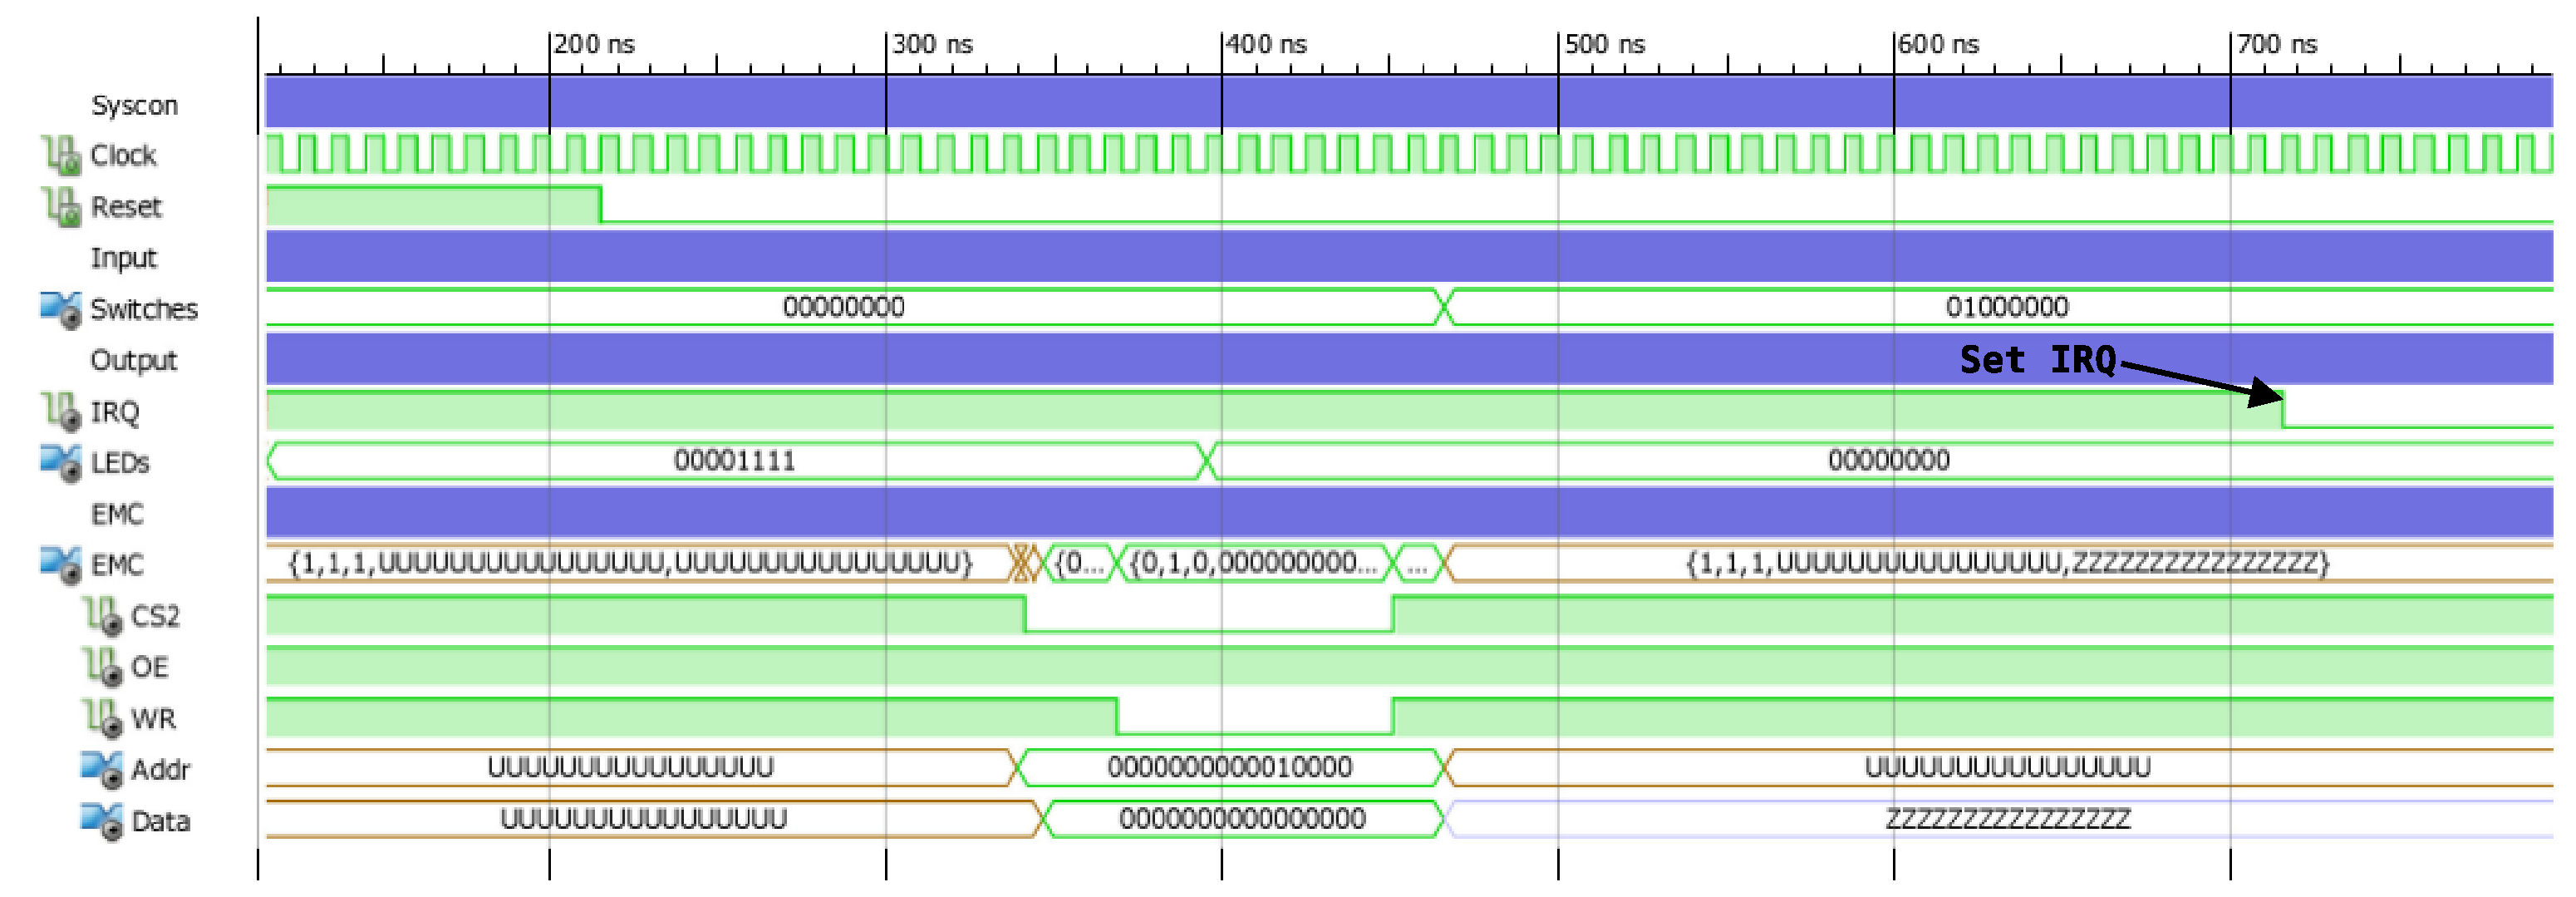
\includegraphics[width=1.0\textwidth]{images/tb7_BFM_write.eps}
		\caption{BFM write}
	\end{centering}
\end{figure}
The figure below is the continued BFM test bench. First the BFM reads the interrupt register, the first arrow shows when the data is valid on the Spartan 6, the blue maker indicate when the EMC is reading data from the Spartan 6. The second arrow shows that the interrupt is deactivated as the interrupt register is read. Next the BFM read the switch register to get the switch position, the arrow again shows when the data is valid, and the blue marker show when the data is read. Last the LEDs is set to the new switch position by another write to the LEDs from the BFM.
\begin{figure}[H]
	\begin{centering}
		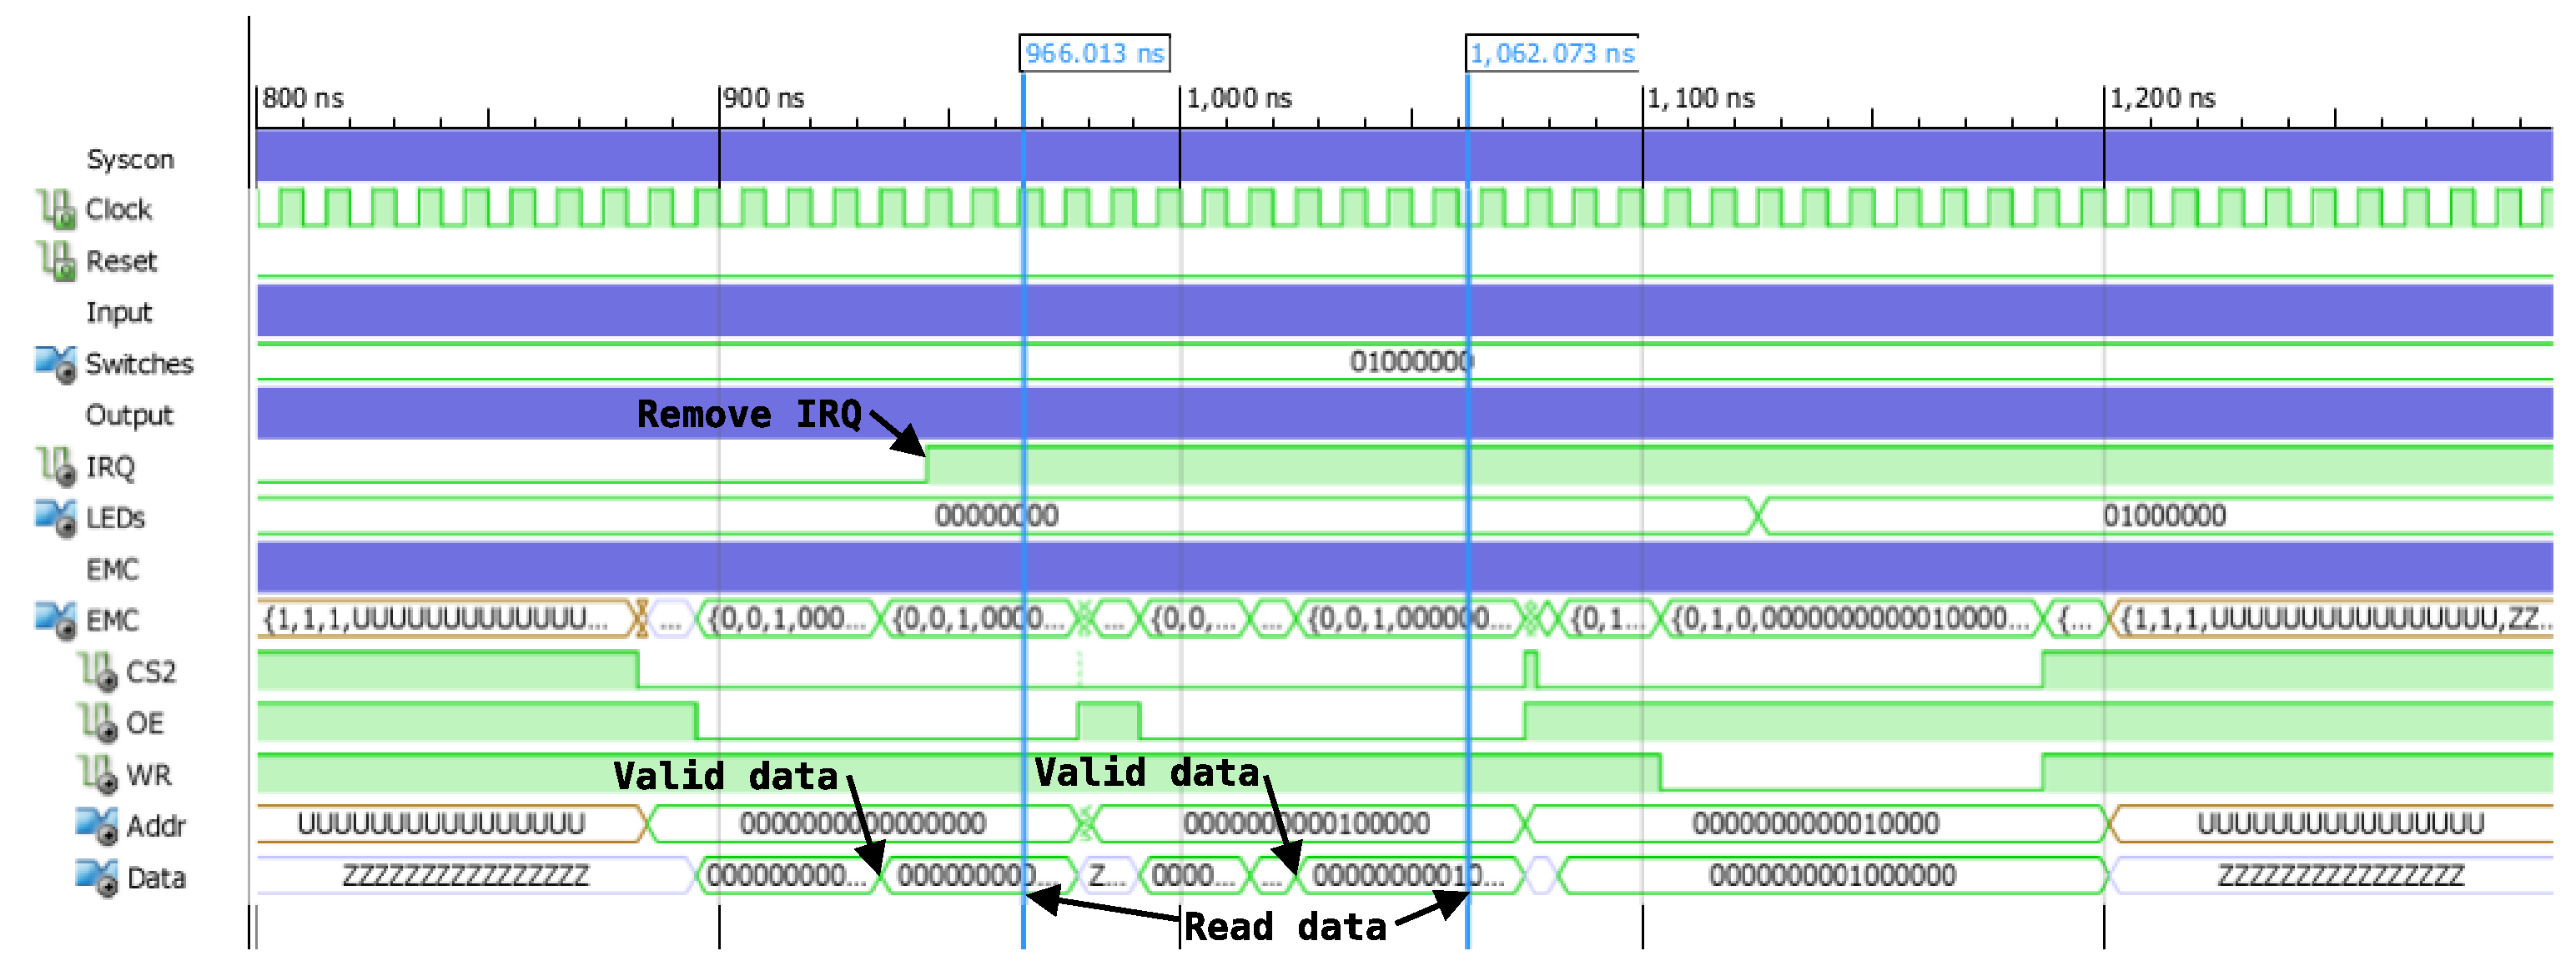
\includegraphics[width=1.0\textwidth]{images/tb7_BFM_read_irq.eps}
		\caption{BFM read IRQ}
	\end{centering}
\end{figure}
\subsubsection{Digital clock manager}
In the code handed out by Morten Opprud Jakobsen, there is a DCM\footnote{Digital Clock Manager}. This module is used for making a jitter-free clock, and have the possibility to change the clock speed in order to match the clock for the LCP2478. The DCM in Spartan 6 tolerates two types of jitter, \textit{cycle-to-cycle jitter} and \textit{period jitter}. Cycle-to-cycle jitter is the change in clock period from cycle to cycle, the period jitter is the change over millions of clock cycles. The code for the DCM is shown below.
\begin{lstlisting}[language=VHDL, caption=DCM\_SP]
...
	clk_o <= clk_r;

-- DCM instantiation for the system clock.
	DCM_Sys : DCM_SP
	generic map (
		CLKFX_DIVIDE				=> 2,											-- Can be any integer from 1 to 32
		CLKFX_MULTIPLY			=> 2)											-- Can be any integer from 2 to 32
	port map	(
				CLK0				=> clk_s,											-- 0 degree DCM CLK ouptput
				CLKFX				=> clk_r,											-- DCM CLK synthesis out (M/D)
				CLKFB				=> clk_s,											-- DCM clock feedback
				CLKIN				=> clk_i,											-- Clock input (from IBUFG, BUFG or DCM)
				RST					=> '0'												-- DCM asynchronous reset input
				);
...
\end{lstlisting}
The DCM in the Spartan 6 has many different features, one of the features that is used is removing jitter, this is done in the code above. The DCM takes the standard clock input, and the zero phase shifted clock is routed into the clock feedback, for the DCM to compensate for jitter. The DCM is also used to scale the clock to match the clock in the LPC2478, this is done by multiplying and dividing the clock with integer values.
\subsubsection{Spartan 6}
The final design of the Spartan 6 in this project has been verified and the figure below shows the top layer block, and the inputs and outputs on the Spartan 6.
\begin{figure}[H]
	\begin{centering}
		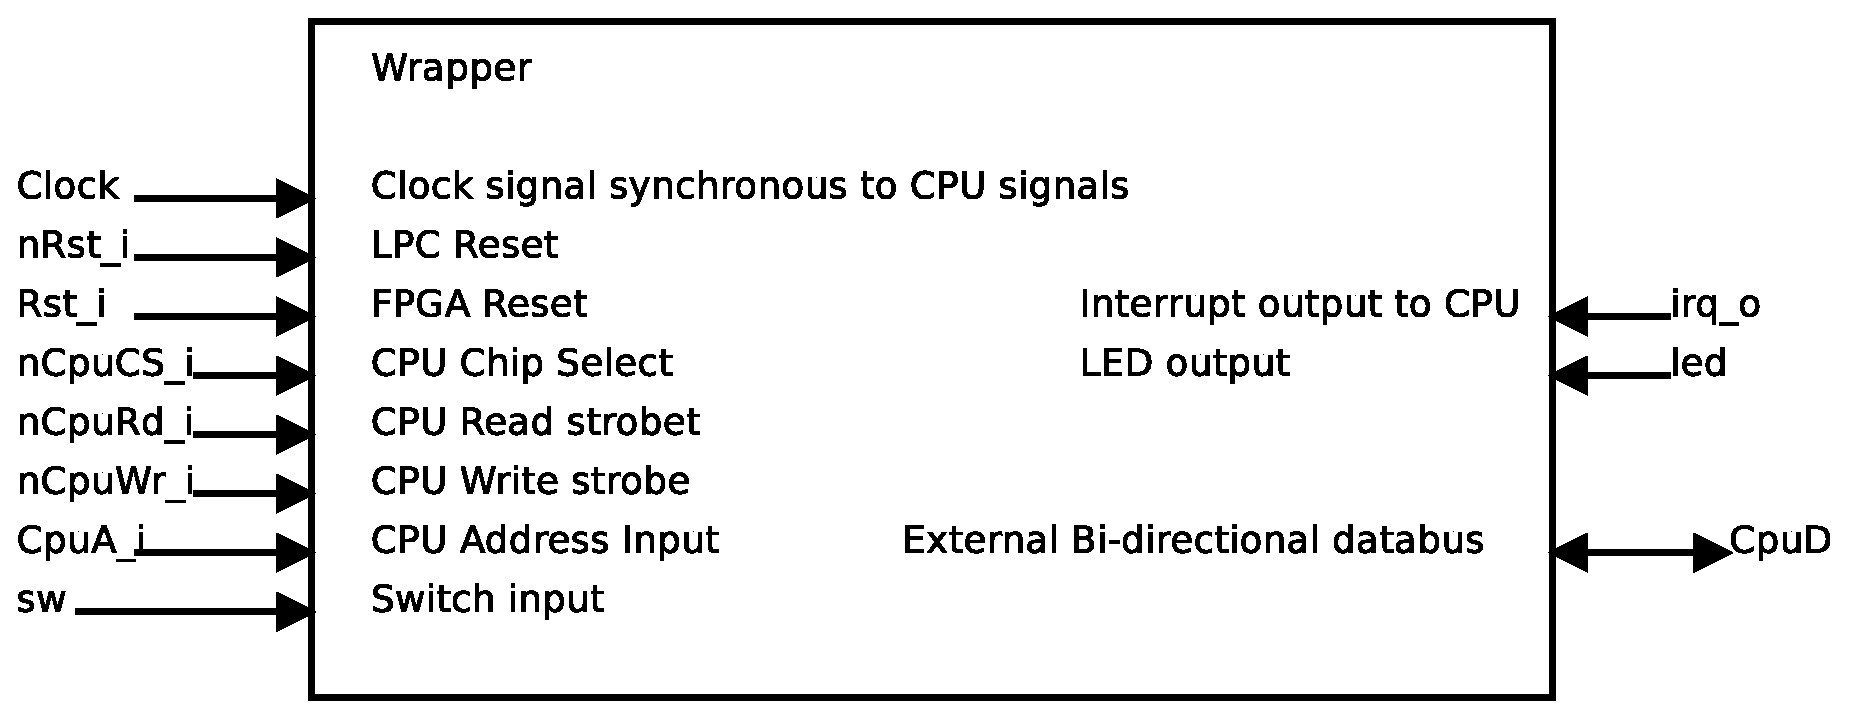
\includegraphics[width=0.9\textwidth]{images/tb7_wrapperblock.eps}
		\caption{Top level in Spartan 6}
	\end{centering}
\end{figure}
The Spartan 6 acts as a memory block seen from the EMC in the LPC2478, the memory map for the Spartan 6 is shown below, with slave addresses, data direction and data length.
\begin{table}[H]
    \begin{tabular}{|l|l|l|l|l|l|p{3.7cm}|}
        \hline
        Name         & DIR		 & S select 	& S address 	& Data                & EMC address & Note                                  \\ \hline
        IRQ Register & Read      & 000          & 0000          & 7 bit - 6 down to 0 & 0x82000000        & Hold data from the interrupting slave \\ \hline
        LED          & Write     & 001          & 0000          & 8 bit - 7 down to 0 & 0x82000020        & Set states of LEDs                    \\ \hline
        Switch       & Read      & 010          & 0000          & 8 bit - 7 down to 0 & 0x82000040        & Hold state of switches                \\
        \hline
    \end{tabular}
    \caption{Memory map of Spartan 6\\
    		 S = Slave, DIR = Direction}
\end{table}
\subsubsection{Conclusion}
The BFM verifies the design. Afterward the design has been tested on the hardware and it is working properly. It is not possible to measure the clock speed with the equipment at the university, so it is not possible to verify that the code fails without the DCM because of jitter on the clock.
% % % % % % % % % % % % % % % % % % % % % % % % % % % % % % % % % % % % % % % % %
% % % % % % % % % % % % % % % % % % % % % % % % % % % % % % % % % % % % % % % % %
% Jesus Thing
% % % % % % % % % % % % % % % % % % % % % % % % % % % % % % % % % % % % % % % % %
\subsection{Power Switch System- Paulo Fontes}
The power switch system is the main functionality of the energy hub, it have to be able to switch the energy flow direction and turn off the port if needed. A prototype PCB was designed in time box 5, in this time box the verifications are made and the PCB is improved according to the results.
\p
Verifications:
\begin{table}[H]
\centering
	\begin{tabular}{| c | l | p{7cm} | }
		\hline
		ID & Description & Verification \\\hline
		1 & Switch the voltage as input or output & Using an mBed to drive the input pins from the power switch system high or low. \\\hline
		2 & Over voltage and under voltage are kept between 30V $ \pm10\% $ & Connect two 30V power supplies in series and decrease the voltage below 27V, and increase again to 30V. Increase the voltage above 33V, and decrease to 30V again. \\\hline
		3 & Current between maximum 30A & Not tested \\\hline
		4 & Current Sensor giving feedback voltage & The current sensor feedback pin is connected to the analogue input in the mBed, the value is shown by the serial connection. \\\hline
	\end{tabular}
\end{table}

Verification 3 is not performed since this board is a prototype, the header pins soldered and the tracks are not consistent to such current and this test could damage the components in the board. For this requirement to be fulfilled the tracks on the PCB should be increase and connectors that could support high currents have to be used.

\subsubsection{Verification}
The verifications are done following the numeration in ID.

\paragraph{Verification ID: 1}
\begin{table}[H]
\centering
	\begin{tabular}{| c | l | p{7cm} | }
		\hline
		ID & Description & Verification \\\hline
		1 & Switch the voltage as input or output & Using an mBed to drive the input pins from the power switch system high or low. \\\hline
	\end{tabular}
\end{table}

The mBed is used to simulate the control system, it will set the input pins from the power switch module high and low according to the commands given to the mBed by serial connection.

\paragraph{Test bench set up:} An variable power supply (0-60V) with max. 1A is used as supply to the system, the mBed will simulate the control system of the power switch system and the voltmeters will show the energy flow direction.
% %	Image of the set up
\begin{figure}[H]
	\begin{centering}
		%\missingfigure{Case 2 Schematics changed}
		\includegraphics[width=0.7\textwidth]{images/tb7_ps_setup.png}
		\caption{Test bench set up}
	\end{centering}
\end{figure}

The code implemented in the mBed uses 3 pins, a regulated 5V is supplied to the current sensor and the USB serial connection is used for the communication. Pins 13 and 14 are set as digital outputs while pin 15 is set as analogue input for the current sensor measure.

\paragraph{Case scenario 1:} Setting the output pin as high, will drive the SHTD pin high, closing the circuit. The energy will flow from the power line (source) to the module (load). Using a voltmeter the input voltage and output voltage is measure and a drop of 10mV. The results are as expected.

% %	Image of the set up 1
\begin{figure}[H]
	\begin{centering}
		%\missingfigure{Case 2 Schematics changed}
		\includegraphics[width=0.7\textwidth]{images/tb7_ps_case1.png}
		\caption{Case scenario 1: Energy flow from power line to the module}
	\end{centering}
\end{figure}


\paragraph{Case scenario 2:}Changing, the input pin to high and the output pin low, energy will not flow in any direction since the circuit will be open from source to load and two MOSFETs back to back will work as a diode. The results are as expected.

% %	Image of the set up 2
\begin{figure}[H]
	\begin{centering}
		%\missingfigure{Case 2 Schematics changed}
		\includegraphics[width=0.7\textwidth]{images/tb7_ps_case2.png}
		\caption{Case scenario 2: Open circuit energy is blocked by the back to back MOSFETs working as diode.}
	\end{centering}
\end{figure}

Both ports are tested and the system works as expected. The tests show that the system have a low voltage drop across the MOSFETs but still working as a diode. The direction of the energy flow can be changed without problems. The verification is successful.

\paragraph{Verification ID: 2}
In this verification both ends of the systems are tested for over and under voltage. The power supply is connected and the voltage in increased until 35V, after its estabelized again at 30V and decreased to 25V. The power switch system should shut down the port if over 33V and under 25V.

\begin{table}[H]
\centering
	\begin{tabular}{| c | l | p{7cm} | }
		\hline
		ID & Description & Verification \\\hline
		2 & Over voltage and under voltage are kept between 30V $ \pm10\% $ & Connecting two 30V power supplies in series and decrease the voltage below 27V and increase again to 30V until stabilise. Increase the voltage above 33V, and decrease to 30V again. \\\hline
	\end{tabular}
\end{table}

The test bench used is the same as in the earlier verification.

\paragraph{Case scenario 1:} The power supply is connected to the power line, the voltage is increased to 34V.

% %	Image of the set up 1
\begin{figure}[H]
	\begin{centering}
		%\missingfigure{Case 2 Schematics changed}
		\includegraphics[width=0.7\textwidth]{images/tb7_ps_ov_1.png}
		\caption{Case scenario 1: Voltage above 33V will shut down the port.}
	\end{centering}
\end{figure}

\paragraph{Case scenario 2:} The power supply is connected to the power line, the voltage is decrease to 26V.

% %	Image of the set up 2
\begin{figure}[H]
	\begin{centering}
		%\missingfigure{Case 2 Schematics changed}
		\includegraphics[width=0.7\textwidth]{images/tb7_ps_ov_2.png}
		\caption{Case scenario 2: Voltage below 27V will shut down the port.}
	\end{centering}
\end{figure}

The results were the same in both ports, this verification shows that the system have a low and high voltage protection as requested in common requirements. The under voltage protection is unnecessary and might even give malfunctions to the system, since the system might be running only on the power provided by a battery module at the time the voltage goes under 27V, this will shut down the port and the system will be disconnected from any power source. 

\paragraph{Verification ID: 4}
The current sensor implemented in the power switch system is used to retrieve data regarding the direction of the flow and for security reasons turn of the port in case the current is too high. For this test a variable load is added to the test bench and set to 30$\omega$. The current sensor implemented gives a feedback of 40mV/A.

\begin{table}[H]
\centering
	\begin{tabular}{| c | l | p{7cm} | }
		\hline
		4 & Current Sensor giving feedback voltage & The current sensor feedback pin is connected to the analogue input in the mBed, the value is shown by the serial connection. \\\hline
	\end{tabular}
\end{table}

\paragraph{Case scenario 1:} The power supply is connected to the power line and a variable load as module. The resistance is set to 30$\omega$ giving a difference of approximately 40mV in the feedback pin.

% %	Image of the set up 1
\begin{figure}[H]
	\begin{centering}
		%\missingfigure{Case 2 Schematics changed}
		\includegraphics[width=0.7\textwidth]{images/tb7_ps_cs_1.png}
		\caption{Case scenario 1: Current measures.}
	\end{centering}
\end{figure}

Due to the sensitivity of the current sensor, the accuracy can change according to the temperature and voltage supplied. Improvements regarding the accuracy have to be done.

\subsection{Web Interface - Paulo Fontes}
For the development and evaluative procedures, a LAMP(Linux Apache MySQL PHP) web server is set up, this process is described in time box 4. The web interface can be accessed on the university network at the address http://10.1.18.223/.
\p
The web interface application includes a great amount of different scripting languages such as server side PHP and client side JavaScript, along with markup languages HTML and XML. The code for each will not be explained extensively, instead the most important functionalities will be filtered and explained.
\p
An extra web application is developed in PHP only for evaluative propose, it allows the user to view the code of all the files on the web server file structure. By this method the last version of the code is always updated for visualization. The application is called SeeIt and can be accessed at the address: http://10.1.18.223/SeeIt/. 

%			Intro
%					verification specification
%					deployment specification
%
\subsubsection{Analysis}

\paragraph{Database}
For a well constructed database, it has to be consistent, flexible and efficient so no data is lost or repeated when saved. The data base structure has changed since time box 4 when it was developed. The new structure can be seen bellow.

TYPE(ID\_TYPE, NAME);

\begin{table}[H]
\centering
	\begin{tabular}{| p{2cm} | p{10cm} |}
		\hline
		ID\_TYPE & Auto increment integer, a new id number is generated when a different type is needed to the system. \\\hline
		NAME & Describe the type name for example: Input, output, bidirectional, etc.\\\hline
	\end{tabular}
\end{table}

STATUS(ID\_STATUS, NAME);

\begin{table}[H]
\centering
	\begin{tabular}{| p{2cm} | p{10cm} |}
		\hline
		ID\_STATUS & Auto increment integer, a new id number is generated when a different status is needed to the system. \\\hline
		NAME & Describe the status name for example: Running, stopped, warning, etc.\\\hline
	\end{tabular}
\end{table}


MODULES(ID\_MODULE, ID\_TYPE, NAME, HUB\_PORT);

\begin{table}[H]
\centering
	\begin{tabular}{| p{2cm} | p{10cm} |}
		\hline
		ID\_MODULE &  Module unique ID, this id as primary key ensures that no module with is repeated in the database.\\\hline
		ID\_TYPE & This is a foreigner key for the table type, this way if some other type of module is needed it can be dynamical add. \\\hline
		NAME & The name of the module for example, Solar Panel, wind turbine, battery. \\\hline
		HUB\_PORT & Actual connected port for this module\\\hline
	\end{tabular}
\end{table}

As a requirement, the database have to store the measurement  from different sensors. This is stored in a the table MEASUREMENTS.

MEASUREMENTS(ID\_MEASURE, ID\_SENSOR, DATE\_TIME, HUB\_PORT, VALUE)

\begin{table}[H]
\centering
	\begin{tabular}{| p{2cm} | p{10cm} |}
		\hline
		ID\_MEASURE &  Measurement id, auto increment field.\\\hline
		ID\_SENSOR & This is a foreigner key for the table sensor, this associated the value retrieved to the correspondent sensor. \\\hline
		DATE\_TIME & Date and time of the measurement is saved so it can be plotted or in case of a lower efficiency a detailed history can analysed. \\\hline
		HUB\_PORT & Actual connected port for this module\\\hline
		VALUE & Measurement retrieved by the energy hub.\\\hline
	\end{tabular}
\end{table}

Logs are a simplified method of keeping track about what is happening in the system, this is one of the most fundamental functionalities of the system.

LOGS(ID\_LOG, ID\_MODULE, DATE\_TIME, ID\_STATUS, ID\_USER, ID\_ERROR);

\begin{table}[H]
\centering
	\begin{tabular}{| p{2cm} | p{10cm} |}
		\hline
		ID\_LOG & Auto increment integer, a new id number is generated every time a measurement is add. \\\hline
		ID\_MODULE & This is a foreigner key for the table modules, this allow the system to know from which module correspond the measurement .\\\hline
		DATE\_TIME & Date and time of the log is saved, in case of malfunction it will help with a time line. \\\hline
		ID\_STATUS & The new status of the module that was changed.\\\hline
		ID\_USER & Foreigner key for the table users, this will allow the system to know which user made the change. \\\hline
		ID\_ERROR & Foreigner key for the table error, if any error occurs it will be stored. \\\hline
	\end{tabular}
\end{table}

For error handling situations a table ERRORS is created this way the administrator can have more control and act in case some mall function of the system.
\\\\

ERRORS(ID\_ERROR, NAME);

\begin{table}[H]
\centering
	\begin{tabular}{| p{2cm} | p{10cm} |}
		\hline
		ID\_ERROR & Auto increment integer, a new id number is generated when a different unit is needed to the system. \\\hline
		NAME & Predefined error description. \\\hline
	\end{tabular}
\end{table}

Measurements are add to the database constantly, which in a non-stop system database size could be a problem, to avoid this situation a MERGES data set is created. This will store an average of values between a time span for each sensor, allowing the customer either to erase the values from the log or export them out from the database.
\\\\

MERGERS(ID\_MERGE, DATE\_FROM, DATE\_TO, ID\_SENSOR, VALUE);

\begin{table}[H]
\centering
	\begin{tabular}{| l | p{10cm} |}
		\hline
		ID\_MERGE & Auto increment integer, a new id number is generated every time an wrap is needed. \\\hline
		ID\_SENSOR & This is a foreigner key for the table sensors, this allow the system to know from which sensor correspond the values .\\\hline
		DATE\_FROM & Date and time of the time span start. \\\hline
		DATE\_TO & Date and time of the time span end. \\\hline
		VALUE & Average measurements value. \\\hline
	\end{tabular}
\end{table}

SENSOR(ID\_SENSOR, ID\_MODULE, ID\_UNITS);

\begin{table}[H]
\centering
	\begin{tabular}{| p{2cm} | p{10cm} |}
		\hline
		ID\_SENSOR & Auto increment integer, a new id number is generated when a different sensor is needed to the system. \\\hline
		ID\_MODULE & This is a foreigner key for the table sensors, this allow the system to know from which module correspond the sensor, being a primary key with the id\_sensor, this way each sensor correspond to only one module .\\\hline
		ID\_UNITS & This is a foreigner key for the table units, this allow the system to know which units the sensor is measuring.\\\hline
	\end{tabular}
\end{table}

UNITS(ID\_UNIT, NAME);

\begin{table}[H]
\centering
	\begin{tabular}{| p{2cm} | p{10cm} |}
		\hline
		ID\_UNIT & Auto increment integer, a new id number is generated when a different unit is needed to the system. \\\hline
		NAME & Describe the unit name for example: A, V, deg ,m/s,etc. (Ampere, Volt, Degrees, Velocity)\\\hline
	\end{tabular}
\end{table}
To increase security, an USERS table is added associated with different PRIVILEGES for different users. A user root is created leaving the system able to manage multiple users with different privileges if needed.
\\

USERS(ID\_USER, NAME, PASS, EMAIL, ID\_PRIV);

\begin{table}[H]
\centering
	\begin{tabular}{| p{2cm} | p{10cm} |}
		\hline
		ID\_USER & Auto increment integer, a new id number is generated when a different privilege is needed to the system. \\\hline
		NAME & Username credential. \\\hline
		PASS & User password (Not encrypted in this version). \\\hline
		EMAIL & Email to which warnings are send. \\\hline
		ID\_PRIV & Foreigner key for the table privileges. \\\hline
	\end{tabular}
\end{table}

PRIVILEGES(ID\_PRIV, NAME);

\begin{table}[H]
\centering
	\begin{tabular}{| p{2cm} | p{10cm} |}
		\hline
		ID\_UNIT & Auto increment integer, a new id number is generated when a different privilege is needed to the system. \\\hline
		NAME & Describe the user privileges. \\\hline
	\end{tabular}
\end{table}
For the communication process between the web interface and the energy hub, the ip address of the device need to be always accessible this way a table DEVICES is created in which the last known IP address of the device is stored.
\\\\

DEVICES(ID\_DEVICE, IP);

\begin{table}[H]
\centering
	\begin{tabular}{| p{2cm} | p{10cm} |}
		\hline
		ID\_DEVICE & Auto increment integer, a new id number is generated when a different ip added. \\\hline
		IP & IP address of the device. \\\hline
	\end{tabular}
\end{table}

At this point, in an abstract way, the database can initialise a new module or identify if the module where connected before, change the status for each module and add new measurements for each sensor.
\paragraph{Data Model}
Data model is a high-level overview of the database structure. At this stage data sets are translated to a logic structure with the relationship between tables.

\begin{figure}[H]
	\begin{centering}
		%\missingfigure{Webserver first page}
		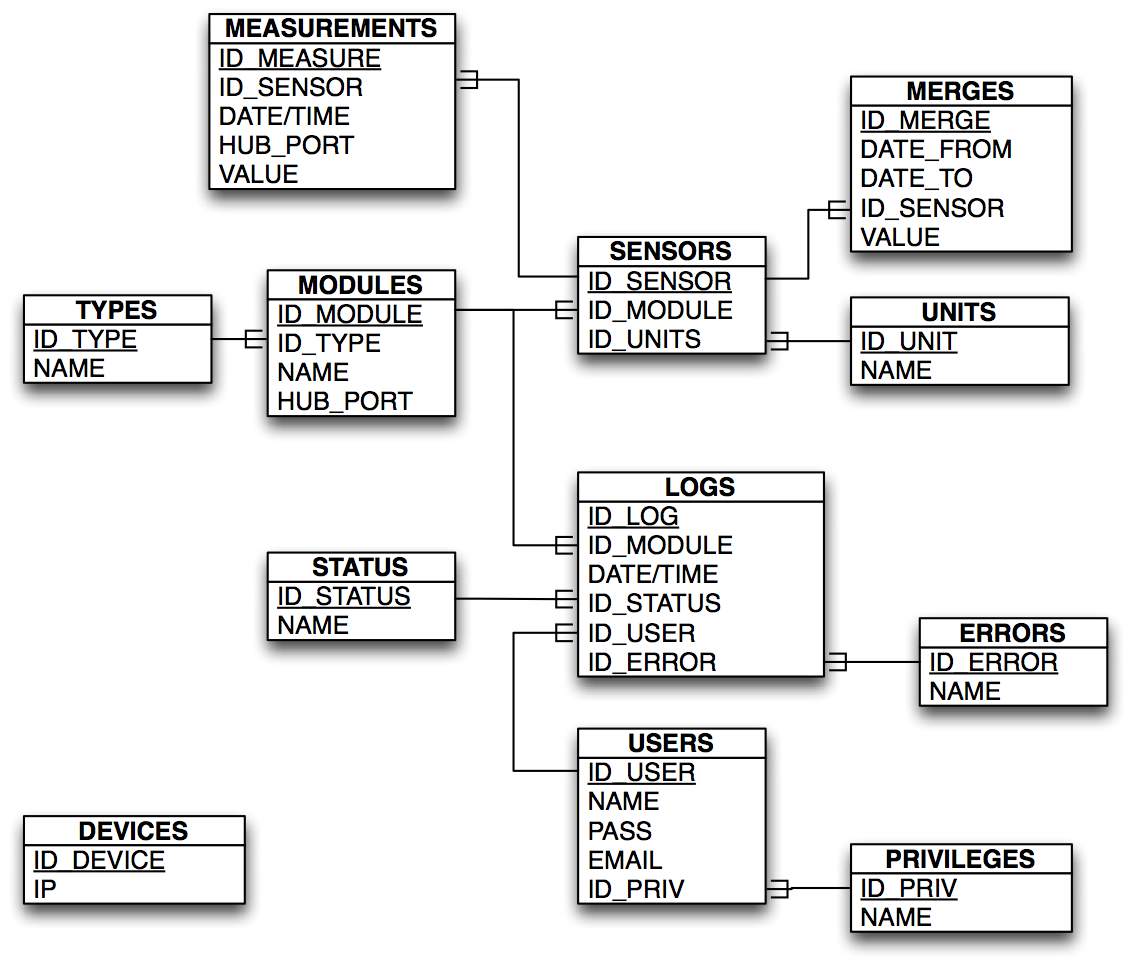
\includegraphics[width=1.0\textwidth]{images/db_datamodel.png}
		\caption{Database relational overview ( Data Model )}
	\end{centering}
\end{figure}

\paragraph{getData.php} This script is described in this section since its main functionality is to retrieve values from the database using SQL queries and construct a XML file with the data retrieved. Only the Ampere measurements are requested and saved into this database since this is prototype of the system the necessary protocol and structure for the sensors in the modules was not defined.

Script parameters:
\begin{itemize}
	\item unique\_id - this is the only parameter expected by this script, since it will retrieve all the measurements from an unique module/sensor, the URL encoding method for this parameter have to be POST.
\end{itemize}

Several requests to the database are done by this script, each SQL query and is described bellow:

Current power production of the modules:
\begin{lstlisting}[language=sql]
// Current Power Production and Current Power Consuption
	$sql = "SELECT  VALUE FROM `MEASUREMENTS` WHERE `ID_SENSOR`=".$_POST['unique_id']." ORDER BY ID_MEASURE DESC LIMIT 1";
	$res = $con->query($sql);
	$row = $res->fetch_row();
	if($row[0]>0){
		$c_pw_pro = ($row[0]*$voltage)."W ";
		$c_pw_con = "0W ";
	} else if ($row[0]<0){
		$c_pw_con = ($row[0]*$voltage*-1)."W ";
		$c_pw_pro = "0W ";
	} else {
		$c_pw_pro = "0W ";
		$c_pw_con = "0W ";
	}
\end{lstlisting}

The SQL query, uses the keyword \textbf{SELECT} to show the value of the column \textbf{VALUE}, \textbf{FROM} the table \textbf{MEASUREMENTS}, \textbf{WHERE} the field \textbf{ID\_SENSOR} match with the \textbf{unique\_id} send by parameter, the results are \textbf{ORDER BY} the column \textbf{ID\_MEASURE}, from the last inserted value to the first(\textbf{DESC}), with a \textbf{LIMIT} of \textbf{1} result.

The result of this query is the last data entry in the table. If the value is negative it will be multiplied by the voltage and -1, this is the current power consumption. If positive it will be multiplied by the voltage and assigned to the current power production.

Total Power Production:
\begin{lstlisting}
	$sql = 'SELECT SUM(VALUE) 
			FROM `MEASUREMENTS` 
			WHERE `ID_SENSOR`='.$_POST['unique_id'].'
			AND DATE_TIME>(SELECT DATE_TIME FROM LOGS WHERE ID_MODULE='.$_POST['unique_id'].' ORDER BY DATE_TIME DESC LIMIT 1)';
	$res = $con->query($sql);
	$row = $res->fetch_row();
	$tt_pw_pro = ($row[0]*$voltage)."W ";
\end{lstlisting}

The SQL query, uses the keyword \textbf{SELECT} to retrieve the addition (\textbf{SUM}) of the values from the column \textbf{VALUE}, \textbf{FROM} the table \textbf{MEASUREMENTS}, \textbf{WHERE} the field \textbf{ID\_SENSOR} match with the \textbf{unique\_id} send by parameter, AND the columns DATE\_TIME is greater than the result from the  \textbf{SELECT} value of the field \textbf{DATE\_TIME FROM} table LOGS \textbf{WHERE} the \textbf{ID\_SENSOR} match with the \textbf{unique\_id} send by parameter, this result is \textbf{ORDER BY} the column \textbf{DATE\_TIME}, from the last inserted value to the first(\textbf{DESC}), with a \textbf{LIMIT} of \textbf{1} result.

This query returns the addition of all data in column VALUE from the table measurements after the date and time of the last log entry. This way the total power production seen in the user interface corresponds to the uptime of the module/sensor.

Average power production:
\begin{lstlisting}[language=sql]
	// Average Power Production
	$sql = 'SELECT AVG(VALUE) 
			FROM `MEASUREMENTS` 
			WHERE `ID_SENSOR`='.$_POST['unique_id'].'
			AND DATE_TIME>(SELECT DATE_TIME FROM LOGS WHERE ID_MODULE='.$_POST['unique_id'].' ORDER BY DATE_TIME DESC LIMIT 1)';
	$res = $con->query($sql);
	$row = $res->fetch_row();
	$avg_pw_pro = ($row[0]*30)."W ";
\end{lstlisting}

This query is similar to the total power production, instead of the addition of the data in the column VALUES the average is made. This will give the average of values since the last data entry in the table logs.

Module status:
\begin{lstlisting}[language=sql]
	// Status
	if($_SESSION['error_device']==1){
		$stat = "Connection Failed";
	} else {
	
	$sql = 'SELECT `STATUS`.NAME, `STATUS`.ID_STATUS
			FROM STATUS 
			INNER JOIN LOGS ON `STATUS`.ID_STATUS = `LOGS`.ID_STATUS
			WHERE `ID_MODULE`='.$_POST['unique_id'].'
			ORDER BY `LOGS`.ID_LOG DESC 
			LIMIT 1';
	
	$res = $con->query($sql);
	$row = $res->fetch_row();
	
	if($row[0]==""){
		$stat = "Disconnected";
		$id_stat = 2;
	} else {
		$stat = ($row[0]);
		$id_stat = $row[1];
	}
	
	if($row[1]!=3){
			$uptime = " --- ";
			$c_pw_pro = " --- ";
			$c_pw_con = " --- ";
			$tt_pw_pro = " --- ";
			$avg_pw_pro = " --- ";
	} ...
\end{lstlisting}

The SQL query, uses the keyword \textbf{SELECT} to show the values of the columns \textbf{NAME} and \textbf{ID\_STATUS}, \textbf{FROM} table \textbf{STATUS}, when joined (\textbf{INNER JOIN ON}) with table \textbf{LOGS} where the \textbf{STATUS.ID\_STATUS} match with \textbf{LOGS.ID\_STATUS}, and \textbf{WHERE} the field \textbf{ID\_MODULE} match with the \textbf{unique\_id} send by parameter, the results are \textbf{ORDER BY} the column \textbf{ID\_LOG}, from the last inserted value to the first(\textbf{DESC}), with a \textbf{LIMIT} of \textbf{1} result.

This query returns the status name and id for the desired module, the returned values are assigned to the variable stat and id\_stat for later use in this script. In case the status id is different then 3, the module will not be running, so no values are shown to the user.

Create the XML result:
\begin{lstlisting}[language=sql]
	echo '<DATA>'.
			 '<C_PW_PRO>'.$c_pw_pro.'</C_PW_PRO>'.
			 '<C_PW_CON>'.$c_pw_con.'</C_PW_CON>'.
			 '<TT_PW_PRO>'.$tt_pw_pro.'</TT_PW_PRO>'.
			 '<AVG_PW_PRO>'.$avg_pw_pro.'</AVG_PW_PRO>'.
			 '<UPTIME>'.$uptime.'</UPTIME>'.
			 '<STAT id_stat="'.$id_stat.'">'.$stat.'</STAT>'.
			 '<M1 id="'.$m_id[1].'" name="'.$m_name[1].'" status="'.$m_status[1].'" id_status="'.$m_id_status[1].'"></M1>'.
			 '<M2 id="'.$m_id[2].'" name="'.$m_name[2].'" status="'.$m_status[2].'" id_status="'.$m_id_status[2].'"></M2>'.
			 '<PRIV>'.$priv.'</PRIV>'.
			 '<DEV_ERROR>'.$_SESSION['error_device'].'</DEV_ERROR>'.
			'</DATA>';
\end{lstlisting}
XML as HTML is a markup language, using elements defined by tags. JavaScript is able to translate XML files with built-in objects, this allows the return of a large amount of data at once, reducing the number of scripting needed and requests to the web server.

The construction of the XML file can be seen above, the main element is DATA, having several 'child nodes'. This nodes (like HTML) can have several attributes, for example the element M1 and M2 contain attributes that defines the modules connected to the port 1 and 2 of the energy hub.

\paragraph{File Structure}
The file structure defines how files are grouped on a system, in a web server architecture the files are stored in the root directory defined by the web server (Apache) configuration. The file structure necessary for this web interface has change since last time box due to a meeting with other teams. The above structure was approved from the meeting.

\begin{figure}[H]
	\begin{centering}
		%\missingfigure{Webserver first page}
		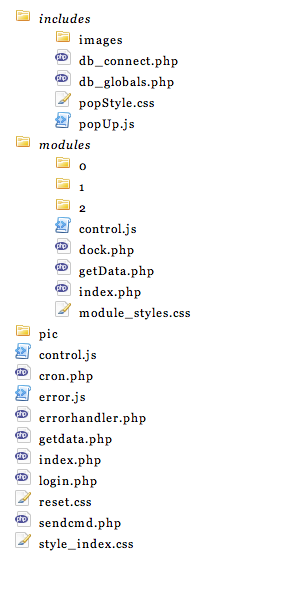
\includegraphics[width=0.3\textwidth]{images/file_structure.png}
		\caption{Proposed File structure}
	\end{centering}
\end{figure}

A short description for each script listed above can be seen in this list:
\begin{itemize}
	\item includes/images/ - Contains images related with the system functionalities.
	\item includes/db\_connect.php - Handle the connection to the MySQL database.
	\item includes/db\_globals.php - Includes all the global variables with the credentials for the database.
	\item includes/popStyle.css - Popup login style definition.
	\item includes/popUp.js - Client side script to handle the user login.
	\item modules/[0-2] - Modules pages, the numbers are associated with the modules ids, being 0 the hub, 1 the battery and 2 the photovoltaic panels.
	\item modules/control.js - Client side script, makes background requests to a PHP script, this script is part of the user experience optimization.
	\item modules/dock.php - PHP script contains the navigation system for the web interface.
	\item modules/getdata.php - PHP script called in background by the client side script running recursively control.js, this script retrieves the system status and data form database in real time, is part of the user experience optimization.
	\item modules/index.php - This page includes each module page structure.
	\item modules/module\_styles.css - Graphical layout definition.
	\item control.js - Client side script, makes background requests to a PHP script and handle the connections of new modules, this script is part of the user experience optimization.
	\item cron.php  - Cron jobs are running by the server in a predefined time, in this case the cron.php at the web server root will point to the cron jobs inside each module folder.
	\item error.js - Client side script, make background requests to a PHP script part of the error handling system.
	\item errorhandler.php - PHP script called in background by the client side script running recursively, is part of the error handling system.
	\item getdata.php - PHP script called in background by the client side script running recursively control.js, this script retrieves the modules connected to the system in real time. Is part of the user experience optimization.
	\item index.php - First page of the web interface.
	\item login.php  - This PHP script is called in background by the pop up login client side script.
	\item reset.css - Layout definition of the web interface.
	\item sendcmd.php - Webservice to send commands to the desired module/enegy hub.
	\item style\_index.css - Layout definition of the web interface.
\end{itemize}

Due to the size of such system and the few time for the development, the project was scaled down so a high fidelity prototype where the system to be can be implemented and the main functionalities of the system tested.

\paragraph{Error Handling}
The web server have to be able to handle errors such the lost of communication with the energy hub or database connection problems. For a reliable system, a script running on the client side using JavaScript have to be implemented, this way the web interface can recursively test the communication to the energy hub and database.
\p
Is necessary to define the web interface response for both situations database and energy hub connection lost. If the connection is lost to the device the user is able to see the data stored in the database, so the system is not blocked, but a warning is shown to the user/administrator, do the correspondent debug can be done. In case the connection to the database is lost, the user interface is blocked with an warning, the energy hub will continue working, since it doesn't affected the correct work of the system to route the energy, in this situation all the data retrieved by the modules will be lost.
\p
Since a script is running recursively at the client side, when the communications are re-establish to the energy hub or database the user will be able to use the system normally, this is a great improvement in the user experience and functionalities as an web application.

\subsubsection{Implementation}
The development of the web interface is made in a local machine using MAMP ( MAC Apache MySQL PHP), and transfer later on to a web server on the university network. 

\paragraph{Communication}
The communication between the several components of the system is crucial, data is retrieved at a high rate from the modules, so an effective communication between the energy hub and the web server is implemented. Among the communication with the energy hub, the web interface needs a constant connection with the MySQL server, so data can added and retrieved from the database.

\paragraph{savedata.php}
A background application running in the energy hub converts the measurement sent through PLC (UART) to a HTTP request \textbf{savedata.php?sensor\_id=ID Sensor\&value=Sensor Measurement\&hub\_port=Hub Port}.

Script parameters:
\begin{itemize}
	\item sensor\_id - Id of the sensor to where save data.
	\item value - the vlue to be saved
	\item hub\_port - the connected port of the module
	\item op - status, change status of a module. <unique\_id><new status>, this is added to the log table.
\end{itemize}
\begin{lstlisting}[language=php]
<?php
	function changeStatus($con){
		$date = getdate();
		$today = $date['year'].'-'.$date['mon'].'-'.$date['mday'].' '.$date['hours'].':'.$date['minutes'].':'.$date['seconds'];
		$sql = 'INSERT INTO `LOGS` (
				`ID_LOG` ,
				`ID_MODULE` ,
				`DATE_TIME` ,
				`ID_STATUS` ,
				`ID_USER` ,
				`ID_ERROR` 
				)
				VALUES (
				NULL , \''.$_GET['id_module'].'\', \''.$today.'\', \''.$_GET['id_status'].'\', \''.$_SESSION['id_user'].'\', \'1\'
				)';
		if($con->query($sql)){
			echo "Success";
		}
		$sql = 'UPDATE `MODULES` SET `HUB_PORT` = '.$_GET['hub_port'].' WHERE `MODULES`.`UNIQUE_ID` ='.$_GET['id_module'];
		
		if($con->query($sql)){
			echo "Success";
		}
	}
	
	if(isset($_GET['op'])){
		
		switch ($_GET['op']){
			case "status": changeStatus($con); break;	
		}
		
	} else {
		$date = getdate();

		$today = $date['year'].'-'.$date['mon'].'-'.$date['mday'].' '.$date['hours'].':'.$date['minutes'].':'.$date['seconds'];

		if(isset($_GET['sensor_id']) && isset($_GET['value']) && isset($_GET['hub_port'])){
			$sql= "INSERT INTO `MEASUREMENTS` (".
				  "`ID_MEASURE` ,".
			  	  "`ID_SENSOR` ,".
			  	  "`DATE_TIME` ,".
			  	  "`HUB_PORT` ,".
			  	  "`VALUE`) ".
			  	  "VALUES (NULL , '".$_GET['sensor_id']."', '".$today."', '".$_GET['hub_port']."', '".$_GET['value']."')";
	
			$con->query($sql); // Run the query in the MySQL server
			echo $sql;
		}	else {
			echo 'Invalide parameters';	
		}
	}
	
?>
\end{lstlisting}

This script saves the measurement retrieved from a sensor to the database. At first it established the connection to the MySQL server so SQL requests can be made.
A PHP function returns an array with the current date and time, this is formatted into YYYY-M-D H:M:S, after it can be saved to the MEASUREMENTS table. The script collects all the parameters send through the URL encoding GET, a SQL code is generated and a request made to the MySQL server, the data is added to the MEASUREMENTS table.
\p
In case of status changes, a parameter \textbf{op} is encode with the method GET and if it value is 'status' the function changeStatus() will be called. This function will update the HUB\_PORT on the table MODULES and insert a new log to the table LOGS. The request for this functionality is  \textbf{savedata.php?op=status\&id\_module=MODULE ID\&id\_status=STATUS TO CHANDE TO\&hub\_port=HUB\_PORT}.

\paragraph{sendcmd.php}

The web interface is able to send commands to the energy hub and the modules using the\\ \textbf{sendcmd.php?id\_module=\textless module id\textgreater\&cmd=\textless command to be send\textgreater }. The id\_module tells the hub which module the command should be send.
No verification is made of the send command by the web server or the energy hub unless the command is specifically send to the hub.

\begin{lstlisting}[language=php]

<?php
	
	// SQL request for the device page.
	require_once("includes/db_connect.php");
	
	if(isset($_GET['cmd']) && isset($_GET['id_module'])){
		
		$device_port = 5555;
			
		$sql= "SELECT IP ". 
			  "FROM `DEVICE` ". 
			  "ORDER BY ID_DEVICE DESC ".
			  "LIMIT 1";
		
		$res = $con->query($sql); // Run the query in the MySQL server
		
		$row = $res->fetch_row();
		
		$device_ip = $row[0];
		
		if (!$socket=socket_create(AF_INET, SOCK_STREAM, SOL_TCP)){
			exit (socket_strerror(socket_last_error()));
		}
	
		if (!socket_connect($socket,$device_ip,$device_port)){
			exit (socket_strerror(socket_last_error()));
		}
	
		$str = $_GET['cmd'].';'.$_GET['id_module'].';'.$_GET['dir'];
		
		socket_write($socket,$str);
	
		$msg='';
		$c='';
    	
		while(socket_recv($socket, $c, 256,0)){
  			if($c != null) {
   				$msg .= $c;
			}
		}
		
		echo $msg;
        
		socket_close($socket);
		
	} else {
		echo 'Command or Module Id not set';
	}

?>
\end{lstlisting}

At first the script will get the ip address of the energy hub, a SQL query retrieves the last IP address added to the table DEVICES. With the energy hub ip and a predefined port, a connection is created using a TCP socket for the communication between the energy hub and the web server. The parameters are collected from the encode URL and translated to a recognized format in the energy hub. The data is send to the energy hub and a answer of success or not is returned.
\p
This script is called in background by a client side script, this will handle how to warning the user in case a problem occurs.

\paragraph{saveip.php}

This script is called by the background application running on the energy hub, it saves the IP address given by DHCP, this is used for further communication between the web server and the energy hub.
\begin{lstlisting}[language=php]
	require_once("includes/db_connect.php");

	if(isset($_GET['ip'])){
		$sql= "INSERT INTO `DEVICE` (".
			  "`ID_DEVICE` ,".
		  	  "`IP`)".
		  	  "VALUES (NULL , '".$_GET['ip']."')";
	
		$con->query($sql); // Run the query in the MySQL server
		
		// No feedback needed since the energy hub will not expect an answer.
		
	} else {
		echo 'IP not set';
	}
\end{lstlisting}
The ip address is send by the GET method (saveip.php?ip=127.0.0.1), this is how the data in encoded into a URL, being collected in the variable \$\_GET['ip']. 
A \$sql variable string is created containing the SQL code to be run at the MySQL server.

\paragraph{db\_connect.php}

For the communication to the database a driver is used in PHP that provides an interface to the MySQL server. The PHP mysqli extension (MySQL improved) is used in this project, this is recommend for MySQL servers version 4.1.3 or later. This extension provides several benefits as a objective-oriented interface, support for multiple statements, embedded server support and more can be found in the MySQL documentation.

\begin{lstlisting}[language=php]
	require_once("db_globals.php");
	
	$con = new mysqli(DB_HOST,DB_USER,DB_PASS,DB_NAME); // Creates new mysql connection
	
	if($con->connect_error){
		echo "Failed to connect to MySQL: (" . $con->connect_errno . " ) ". $con->connect_error;
	} 
	else { echo "Connection established"; }
\end{lstlisting}

In this script an object is instantiated with a connection to the MySQL server.
\p
\textit{\$con = new mysqli\textless parameters \textgreater)}
\p
The parameters are included from the db\_globals.php, setting the server host, user, password and database to be used.

\paragraph{db\_globals.php}

Using a script to define the parameters for the MySQL connection, 
All the scripts that need to use the global parameters for the connection to the MySQL server, should include db\_globals.php as shown in the db\_connect.php above.

\begin{lstlisting}[language=php]
	// MySQL condifuration
	DEFINE ('DB_USER','root');
	DEFINE ('DB_PASS','pass');
	DEFINE ('DB_HOST','localhost');
	DEFINE ('DB_NAME','iEnergy');
\end{lstlisting}

The global parameters the connection to the MySQL server are define in this script.

\begin{itemize}
	\item DB\_USER - Database user name with read, write and execute permissions.
	\item DB\_PASS - Password for the user
	\item DB\_HOST - Hostname for the MySQL server, if running at the same host as the PHP server, localhost or 127.0.0.1 should be used.
	\item DB\_NAME - Database name to connect to.
\end{itemize}

\paragraph{Error Handling}
The implementation of an error handling will keep the web interface more reliable, improve user experience and alert the administrators to a error situation. A error handling PHP script is called in background, this script will test the communication between the web server and the energy hub, and the communication to the MySQL server. As described in the analysis in this report, the user interface is blocked giving the message warning when the communication with the MySQL server is lost and a warning is given to the user when no communication with energy hub is found.

\paragraph{errorhandler.php} The error handler PHP script is included in each web page before any other script, this script is included when a page is loaded and is recursively called in background to test the connections. The script gives a XML response, when called as background so the client side JavaScript can handle the real time warnings to the user. This method can be called as active error handle, since it acts in real time, usually error handling is implemented when is need to do some action, for example retrieve data from database. With this system the user is immediately blocked from doing any action until the situation is solved.
\p
Since this script is included before everything else, the HTML, JavaScript and CSS layout is included in the file. Bellow several code blocks were extracted for and easier explanation, the full code can be seen using the application SeeIt and in the appendix of this report.
\p
At first and most important the database connection have to be tested, as such a connection to the database is attempted. If the connection is successful the database error session variable will be 0. In case of connection failure the error variable will be changed to one and kept until the connection is re established, changing the session error variable to 2. This will tell the client side script that the situation was solved and in the next test the variable is changed to 0 again. This can be seen in the code bellow.
\begin{lstlisting}[language=php]
	
	if ($_SESSION['error_db']>1) { 
		$_SESSION['error_db']=0;
	}

	$_SESSION['error_device']=0;

	// Test DB connection
	require_once("includes/db_globals.php");
	
	$con = mysql_connect(DB_HOST,DB_USER,DB_PASS,DB_NAME);
	
	if(!$con){
		$_SESSION['error_db']=1;
		$error = "Failed to connect to database: ". mysql_error();
	} else {
		if ($_SESSION['error_db']==1){
			$_SESSION['error_db']=2;
		} else {
			$_SESSION['error_db']=0;	
		}
	}
\end{lstlisting}

If no error regarding the database connection is acknowledge, the ip address for the energy hub is retrieved and the connection with the energy hub can be established.

\begin{lstlisting}[language=php]
if($_SESSION['error_db']==0){
		
		$device_port = 5555;
		
		$con = new mysqli(DB_HOST,DB_USER,DB_PASS,DB_NAME);
		
		$sql= "SELECT IP ". 
			  "FROM `DEVICE` ". 
			  "ORDER BY ID_DEVICE DESC ".
			  "LIMIT 1";
		
		$res = $con->query($sql);
		
		$row = $res->fetch_row();
		
		$device_ip = $row[0];
\end{lstlisting}

The SQL statement  \textbf{SELECT IP FROM `DEVICE` ORDER BY ID\_DEVICE DESC LIMIT 1} retrieves the last ip address insert in the table. The keywords ORDER BY ID\_DEVICE DESC will show the last data added and the keyword LIMIT 1, limits the number of values return to only one. The value is then fetched from the result and assigned to the variable device\_ip for later use in the connection.
\p
For the communication to the energy hub a socket have to be created and a connection established. In case of one of this steps don't work (Socket creation and Connection), a error session variable is set to 1, the client side application will catch this error and alert the user for such situation. The socket is closed after testing to leave the connection path open for new tests or commands to be send.

\begin{lstlisting}[language=php]
		if (!$socket=socket_create(AF_INET, SOCK_STREAM, SOL_TCP)){
			$_SESSION['error_device']=1;
		} else {
			$_SESSION['error_device']=0;
		}
	
		if (!socket_connect($socket,$device_ip,$device_port)){
			$_SESSION['error_device']=1;
		} else {
			$_SESSION['error_device']=0;
		}
		
		socket_write($socket,"a");
		
		socket_close($socket);
	
	}
\end{lstlisting}

The error handle client side (JavaScript) and server side (PHP) are developed at the same time, since the cooperation between both is essential for the proper operation of the error handling system.
\p
This block of code is used only by the client side script, it make a request to the errorhandle.php with the encoded URL variable op=d, this block will return an XML response. The client side script then interpret the answer and reacts according to the errors.
\begin{lstlisting}[language=php]
	if(isset($_GET['op']) && $_GET['op']=='d'){
		
		echo '<ERROR>'.
			    '<DB>'.$_SESSION['error_db'].'</DB>'.
				'<DEVICE>'.$_SESSION['error_device'].'</DEVICE>'.
			  '</ERROR>';
		
	} else {
\end{lstlisting}

The else statement in this code indicates that, if the script was not called by the error.js, then it will include the necessary HTML, CSS and JavaScript to the file where it was included.
\p
An example of this situation is found at the index.php, the first lines of this script starts the session and includes errorhandle.php.

\begin{lstlisting}[language=php]
<?php
	session_start();
	
	require_once("errorhandler.php");
	
	require_once("includes/db_connect.php");
?>
\end{lstlisting}

\paragraph{error.js}
This script catches and handle errors in the client side, it uses background requests to the PHP script errorhadle.php. By the XML response it acts according the situation. JavaScript is a dynamic language with a lot of potential, and this is used in detail in this script.Meaningful blocks will be extracted from the code and explained here.
\p
Three functions are part of this script, being two of them for animation to improve the user experience, they are not documented in this section. The remaining function is the mains focus of the error handling system, is called makeTests().
\p
This functions initialize the variables req for the URL request, db\_error and dev\_error that will be assigned with the values returned by the request.
At first the browser is tested to define which HTTP request object to use, the main difference is between IE (version 5 and 6) form Microsoft and the rest ot the browsers, since IE (version 5 and 6) uses an ActiveX object to deal with background requests.
\begin{lstlisting}[language=php]
	var req;
	var db_error;
	var dev_error;
	
	if(window.XMLHttpRequest){
		req	= new XMLHttpRequest();
	} else {
		req = ActiveXObject("Microsoft.XMLHTTP");	
	}
\end{lstlisting}

The open and send methods from the XMLHttpRequest object, are used to send a request to the server. The 'open' method specifies the type of encoding used in the URL (GET or POST) and if the request is synchronous or not. The 'send' method sends the request to the server, parameters are needed in case of POST encoding method. 

\begin{lstlisting}[language=php]
	req.open("GET","/errorhandler.php?op=d",false);
	req.overrideMimeType('text/xml');
	req.send();
	
	var result = req.responseXML;
\end{lstlisting}

The result variable is initialized and the returned XML data is assigned to it, this data is then extracted and used according to the situation. An example of retrieved XML data can be seen bellow:

\begin{lstlisting}[language=xml]
		<ERROR>
			<DB>0</DB>
			<DEVICE>0</DEVICE>
		</ERROR>
\end{lstlisting}

%	IMAGE from ERROR HANDLING database and device
%

Graphical representation of an error in the connection to the database and communication to the energy hub device.
\begin{figure}[H]
	\begin{tabular}{ c c }
		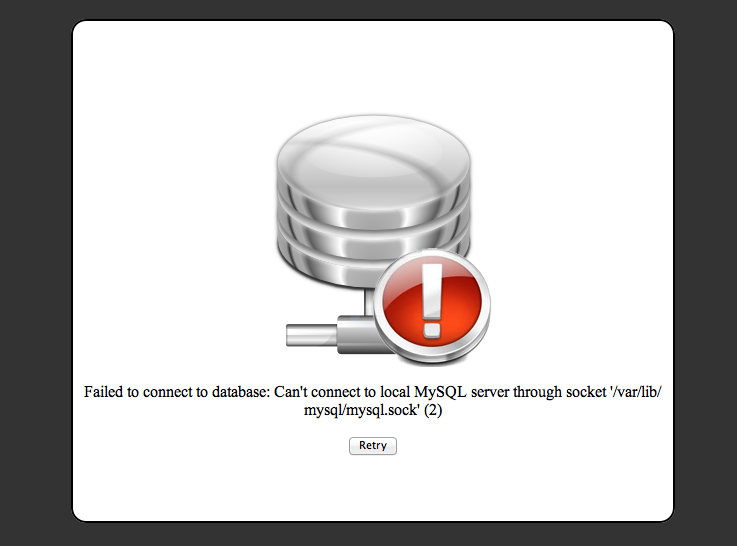
\includegraphics[width=0.5\textwidth]{images/error_db.png}
&
		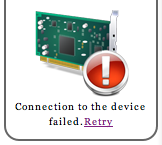
\includegraphics[width=0.2\textwidth]{images/error_device.png}
\end{tabular}
\caption{Database Error and Device communication Error}
\end{figure} 

\subsubsection{Conclusion}

In the analysis phase of this project, it was necessary to understand how can the database an the web interface be verified. As such a scaled down web interface with only two modules and the energy hub is implemented.
\p
With this more realistic approach to the system, it was possible to verify problems regarding the common requirements for the communication between the modules and the energy hub. The database is able to handle several sensors connect to one module, but the energy hub have no knowledge of the sensors connected to each module. For a completely working system, deeper communication and protocol analysis have to be done.
\p
A working high-fidelity prototype is created, ids are assigned to the modules being id:0 to the energy hub, id:1 to the battery and id:2 for the photovoltaic panels. Each module have just one sensor that measures the current (ampere), the id of the sensor is the same as the module id for a working prototype.
\p
The end system can handle all functionalities expected for this project, the energy hub is able to send commands to the energy hub and data can be added or retrieved from the database. The error handling and the dynamic update of contents on the client side, improved the user experience for the control and navigation in the system.
\p 
The web interface is up and running at the address http://10.1.18.223 inside the university network.
% % % % % % % % % % % % % % % % % % % % % % % % % % % % % % % % % % % % % % % % %
% % % % % % % % % % % % % % % % % % % % % % % % % % % % % % % % % % % % % % % % %
% Dennis Thing
% % % % % % % % % % % % % % % % % % % % % % % % % % % % % % % % % % % % % % % % %
\subsection{GPIO Device driver - Dennis}
In order to fulfill the requirements shown in table \ref{tab:gpio_req}\footnote{All requirements can be found in the Appendix EEPRO3}, an driver is needed in order to control the GPIO pins on the micro controller. 
\begin{table}[H]
\centering
	\begin{tabular}{|p{1.2cm}|p{2.8cm}|p{8cm}|p{3.5cm}|}
	\hline
	ID		& Requirement		& Description												& Comments\\\hline
	B-2.1	& Over production & Overproduced energy is wasted in a dummy load connected to the hub. & Energy routing is controlled by GPIO's \\\hline
	B-2.2	& Over production & If two or more producers are connected and one can be without, it is stopped. & Energy routing is controlled by GPIO's \\\hline
	B-2.3	& Under production & If there is no overproduction (dummy load is turned off), the grid is con- nected to the power line in case the producers cannot produce enough energy. & Energy routing is controlled by GPIO's \\\hline
	\end{tabular}
	\caption{Requirements that concerns GPIO}
	\label{tab:gpio_req}
\end{table}
%			Intro
%					verification specification
%					deployment specification
%
\subsubsection{Analysis}
The kernel is running in an embedded system environment with only known parameters connected to it. Therefore a specific GPIO driver is written to decrease development time compared to if a more generic driver was made.
\p 
In order to verify a part
\begin{table}[H]
	\centering
	\begin{tabular}{|p{2cm}|p{2cm}|p{3cm}|p{3cm}|}\hline
		GPIO nr.		& Pin nr.		& Name			& Direction		\\\hline
		GPIO0		& 0.12		& PLC\_nReset		& Output			\\\hline
		GPIO1		& 0.13		& PLC\_wake		& Output			\\\hline
		GPIO2		& 0.18		& PLC\_nSleep		& Output			\\\hline
		GPIO3		& 2.10		& FPGA\_int		& Input Interrupt	\\\hline
		GPIO4		& 1.6			& PS\_main		& Output			\\\hline
		GPIO5		& 1.23		& PS1\_in			& Output			\\\hline
		GPIO6		& 1.25		& PS2\_in			& Output			\\\hline
		GPIO7		& 1.19		& PS1\_out		& Output			\\\hline
		GPIO8		& 1.21		& PS2\_out		& Output			\\\hline
	\end{tabular}
	\caption{GPIO connection table}
	\label{tab:gpio_table}
\end{table}
Table \ref{tab:gpio_table} shows that there will be one device driver with nine valid minor number calls in it. Each of the GPIO devices identifies a GPIO port on the micro controller. The name is an indication of what the GPIO pin is connected to. 
\p \textit{PLC\_nReset}, \textit{PLC\_wake} and \textit{PLC\_nSleep} controls the Power Line Module, by resetting it, wakening it or put it to sleep when there is no need for it.
\p \textit{FPGA\_int} indicates if the FPGA has new data for the micro controller to read, this is indicated by an interrupt.
\p \textit{PS\_main} Turns on or off the supply from the grid.
\p \textit{PS1\_in} and \textit{PS2\_in} sets each of their power switches as an input port whereas \textit{PS1\_out} and \textit{PS2\_out} sets each of their power switch as an output device.        
%			Analysis
%
%                Refactored block diagram
%                Refactored class diagram
%                Detailed use cases
%                User interface specification
%                System interface specification
%                Dimensioning specification 
%
\subsubsection{Design}
When inserting the module the pins needed are configured and given default values. The driver is made so that the pins can be accessed singly and thereby be given a logical value '0' or '1', or a logical value can be read from a single pin.
\p In order to verify if the GPIO device driver works as excepted, the \textit{echo} command and the \textit{cat} commands have been used.
\\ Example of reading GPIO0: \textit{cat /dev/gpio0}
\\ Example of setting GPIO0 to 1: \textit{echo 1 /dev/gpio0}
\p In order to control the power switches an user space application has been written to easy the control of these. The program reads the two first arguments of argv. argv[1] defines the power switch to control, where 0 controls GPIO4 which is the power switch controlling the main. 1 and 2 each controls a power switch connected to a module (wind turbine, battery or similar). argv[2] defines the action of the power switch, where valid arguments are: \textit{in}, \textit{out} and \textit{off}.
\begin{itemize}
	\item in, opens for energy flow from a module to the power line.
	\item out, opens for energy flow from the power line to a module.
	\item off, turns off energy flow in both directions.
\end{itemize}
\begin{lstlisting}[language=c, caption=User space application to control the Power switches]
/*
 ============================================================================
 Name        : port.c
 Author      : E10-Team3 dENNES
 Description : EA-LPC2478 - Control of the power switches connected
 ============================================================================
 */
#define GPIO "/dev/gpio"

/*
        PORT <num> <status>

        Status: in, out, off
        num: 0, 1, 2
        
        in      out
----------------------------
        4       x               PORT0
        5       7               PORT1
        6       8               PORT2
----------------------------
*/


int main(int argc, char *argv[]) {
        	int fd, ret, num;
        	char ibuff[10], obuff[10];
        	char val;	
	char *cmd;
	char dev[3][2]

	num = *argv[1]-'0';
	cmd = argv[2];

        	if(num >= 0 && num <= 2){		// Check if a valid port is called
         		if(strncmp("in", cmd, 2) == 0){	// Set module as input
                   	printf("\nINPUT port%d",num);
                        	dev[num][0] = '1';
                        	dev[num][1] = '0';
                	}
                	else if(strncmp("out", cmd, 3) == 0){	// Set module as output
                       	printf("\nOUTPUT");
                        	dev[num][0] = '0';
                        	dev[num][1] = '1';
                	}
                	else if(strncmp("off", cmd, 3) == 0){	// Turn off module in both directions
                        	dev[num][0] = '0';
                        	dev[num][1] = '0';
                	}
                	else{							// Invalid command sent
                        	printf("\nSomething wrong");
                        	exit(-1);
                	}

                	sprintf(ibuff,"%s%d",GPIO,num+4);	// Compress write string
                	sprintf(obuff,"%s%d",GPIO,num+6);	// ex. /dev/gpio4 if PORT0

                	if((fd = open(ibuff,O_WRONLY)) < 0){	// Open GPIO device driver
                        	printf("Cannot open file in.\n");
                        	exit(-1);
                	}
                	ret = write(fd, &dev[num][0], 1);
                	if(ret < 0){
                        	printf("Write failed in: %d\n", ret);
                        	exit(-1);
                	}
                	close(fd);

                	if(num != 0){					// If port 1 or 2, set second pin on module
                        	if((fd = open(obuff,O_WRONLY)) < 0){
                                	printf("Cannot open file out.\n");
                                	exit(-1);
                        	}
                        	ret = write(fd, &dev[num][1], 1);
                        	if(ret < 0){
                                	printf("Write failed out: %d\n", ret);
                                	exit(-1);
                        	}
                	close(fd);
                	}
        	}
        	return 0;
}
\end{lstlisting}


%       	 Design
%
%                UML/SysML deployment view(s)
%                Mechanical specifications and dimensioning
%                HW module specification per block
%                UML SW deployment view
%                Class specification
%                Refactored class diagram
%                Use case scenarios specifications
%                Sequence diagrams
%
\subsubsection{Implementation}

The gpio header file contains prototypes of the functions used, defines and arrays holding values for the different registers to call in order to avoid \textit{if/else} or \textit{switch/case} in the different functions. 
\begin{lstlisting}[language=c, caption=GPIO header file ]
#define GPIO_MAJOR 245
#define NUM_GPIO_DEVICES 9

#define GPIO_IRQ 14
---
static u32 fdir[] ={
	FIO0DIR,
	FIO0DIR,
	FIO0DIR,
	FIO2DIR,
	FIO1DIR,
	FIO1DIR,
	FIO1DIR,
	FIO1DIR,
	FIO1DIR,
};
---
\end{lstlisting}
The fops (file operations structure) structure with the different device driver call possibilities. This device driver can be opened, closed, read and write.
\begin{lstlisting}[language=c, caption=GPIO fops structure]
static struct file_operations gpio_fops = {
	.owner   	= THIS_MODULE,
	.read			= gpio_read,
	.write  	= gpio_write,
	.open    	= gpio_open,
	.release	= gpio_close,
};
\end{lstlisting}
Initialization of the GPIO pins is called from the init function. The \textit{init} and \textit{exit} functions are similar to the once implemented in the ADC and the UART device drivers except for the \textit{gpioInit} function call.
\begin{lstlisting}[language=c, caption=GPIO init function]
static void gpioInit(void){
	int i=0;
	m_reg_bfs(SCS, 0x1);	// Enable fast I/O on port 0 and 1
	for(i=0 ; i<NUM_GPIO_DEVICES ; i++){
		m_reg_bfc(psel[i], enable_pinsel[i]);
		if(i != 3){
			m_reg_bfs(fdir[i], gpio_pins[i]);
			m_reg_bfs(pin_default_reg[i], gpio_pins[i]);
		}
	}
}
\end{lstlisting}
When the file is opened, the interrupt is configured if it is GPIO3 that is called.
\begin{lstlisting}[language=c, caption=GPIO open function]
static int gpio_open(struct inode* inode, struct file* file){
---
	if(num == 3){
		// setup interrupt for pin input
		DPRINT("\nEnable int for input");
		flag = 0;
		m_reg_bfs(EXTMODE, 1);		// INT0 Edge sensitive
		m_reg_bfc(EXTPOLAR, 1);		// falling edge 
		m_reg_bfs(EXTINT, 1);			// clear pending INT0 interrupts

		ret = request_irq(GPIO_IRQ, interrupt_gpio, SA_INTERRUPT,"GPIO P2.10 interrupt", NULL);
					//SA_SHIRQ 	= Shared interrupt
					//SA_INTERRUPT 	= Fast interrupt

		if(ret){
			printk("IRQ%d is not free. RET: %d\n", GPIO_IRQ, ret);		
			return ret;
		}
	}
	return 0;
}
\end{lstlisting}
The interrupt is freed in the close function if operating in the GPIO3 file.
\begin{lstlisting}[language=c, caption=GPIO close function]
static int gpio_close(struct inode* inode, struct file* file){
---
	if(num == 3){
		free_irq(GPIO_IRQ, NULL);
	}

	return 0;
}
\end{lstlisting}
When read the file returns the character '1' or '0' according to which value the output has. If GPIO3 it read '0' is returned if the pin is low, otherwise the driver is sent to sleep until the pin is '0'. GPIO3 is connected to a pin on the FPGA which is used to symbolize that data is ready to be read from it. The pin goes high again after the external memory address \textit{0x82000000} has been read.
\begin{lstlisting}[language=c, caption=GPIO read function]
static ssize_t gpio_read(struct file *p_file, char *p_buf, size_t count, loff_t *p_pos){
---
	if(num == 3){
		if((m_reg_read(pin_read[num]) & gpio_pins[num]) > 0){
			DPRINT("\nNo interrupt from FPGA, SLEEP!\n");
			m_reg_bfs(PINSEL4, (1<<20));				// Set p2.10 to EINT0
			wait_event_interruptible(my_queue, (flag != 0));	// Put the function to sleep		
			flag = 0;
		}
		value[0] = '0';
	}
	else{
		DPRINT("\nREAD ELSE");
		if((m_reg_read(pin_read[num]) & gpio_pins[num]) > 0){
			value[0] = '1';
		}
		else{
			value[0] = '0';
		}
	}

	if(copy_to_user(p_buf, value, count)){	// Copy read value to user space
		DPRINT("\nFailed: copy_to_user");
		return -EFAULT;
	}
	return 1;
}
\end{lstlisting}
The value written to the device driver shall be a logical '0' or '1' which is then set on the appropriate GPIO pin.
\begin{lstlisting}[language=c, caption=GPIO write function]
static ssize_t gpio_write(struct file *filp, const char *bufp, size_t count, loff_t *p_pos){
---
	if(copy_from_user(value, bufp, count)){	// Copy value from user space to kernel space
		return -EFAULT;
	}
	if(value[0] == '0'){
		//FIO_CLEAR
		DPRINT("\nCLEAR PIN");
		m_reg_bfs(pin_clear[num], gpio_pins[num]);
	}
	else if(value[0] == '1'){
		//FIO_SET
		DPRINT("\nSET PIN");
		m_reg_bfs(pin_set[num], gpio_pins[num]);
	}
	else{
		DPRINT("\nNot a valid character");
		return -EFAULT;
	}

	return count;
}
\end{lstlisting}
If the driver is sent to sleep (in the read function) it jumps to the \textit{interrupt\_gpio} function when awakened as result of the pin having a falling edge.
\begin{lstlisting}[language=c, caption=GPIO interrupt function for GPIO3]
static irqreturn_t interrupt_gpio(int irq, void *dev_id){
	
//	cread = m_reg_read(urbr[0]);		// Read the buffer
	
	DPRINT("\nREAD int\n");	

	m_reg_bfs(EXTINT, 1);		// clear pending INT0 interrupts
	flag = 1;
	wake_up_interruptible(&my_queue);
	return IRQ_HANDLED;
}
\end{lstlisting}

%     	   Implementation
%
%                Mechanical drawings with details explained
%                Electronic diagrams with details explained
%                Source code with details explained
%                Description of integration 
%
\subsubsection{Verification}
In order to test requirement B-2.1, B-2.2 and B-2.3 the whole system needs to be assembled. Table \ref{tab:gpio_req_test} shows the tests described in the Launch phase. 
\begin{table}[H]
\centering
	\begin{tabular}{|p{1.0cm}|p{3.0cm}|p{9.0cm}|p{2.5cm}|}
	\hline
	ID		& Requirement		& Test Description		& Grade/Comment\\\hline
	B-2.1	& Energy Control - Over-Production & A dummy load and a producing module is connected to the system. As no consumers is connected, the system is over- producing. The current flow to the dummy load is measured. If the current flowing to the dummy load is the same as the one coming from the producer (maximum -10\%), the test is valid. &~\\\hline
	B-2.2	& Energy Control - Under-Production & A dummy load and a producing module is connected to the system. As no consumers is connected, the system is over- producing. A variable consuming module is now connected. The resistance in the consuming module is decreased (increas- ing load). The current flow to the dummy load shall now fall. When no current is flowing to the dummy load, it shall be ob- served that the grid is connected. This is done by increasing the load of the consuming module and measuring the current flow from the grid. &~\\\hline
	\end{tabular}
	\caption{Verification of energy routing requirements.}
	\label{tab:gpio_req_test}
\end{table}
As these tests cannot be performed, due to only a part of the system is finish, a minor test has been made in order to verify the functionality of the written device driver.
\p With a multimeter the different pins used as outputs are measured one by one and the output set by sending a value to the file by the \textit{echo} command. Also the pins are read with the \textit{cat} command after setting the pin in order to verify the read function.
\p The interrupt input pin is tested by reading the pin when the FPGA is not yet interrupting to verify if it goes to sleep. If the interrupt pin are read after an interrupt has been given from the FPGA, '0' is returned. 

%       	 Verification
%
%                Module tests
%                Integration tests
%                Acceptance test
\subsubsection{Conclusion}
The small GPIO device driver test has been made with success. All 8 output pins can be set and cleared through the driver. Also the status of the 8 output pins and the one input pin can be read through the driver. If the FPGA has set the interrupt pin to '0', the driver returns '0' immediately without waiting for an falling edge.
% % % % % % % % % % % % % % % % % % % % % % % % % % % % % % % % % % % % % % % % %
% % % % % % % % % % % % % % % % % % % % % % % % % % % % % % % % % % % % % % % % %
% Deployment
% % % % % % % % % % % % % % % % % % % % % % % % % % % % % % % % % % % % % % % % %
\subsection{Deployment}
	%which versions of the prototype the customer will get
	%with what functionality.
\paragraph{Web interface}
The final web interface is up and running at the address http://10.1.18.223 inside the university network.
%
%
\paragraph{GPIO Device driver}
The GPIO driver is working with implemented read and write to single GPIO pins and interrupt on GPIO3. Morten Opprud has been by and verified the functionality.
%
%